\documentclass[lettersize,journal]{IEEEtran}

% ── Core math ────────────────────────────────────────────────────────────────
\usepackage{amsmath,amsfonts,amssymb}
\usepackage{bm}
\usepackage{mathtools}
\usepackage{subcaption}
% ── Algorithms ───────────────────────────────────────────────────────────────
\usepackage{algorithm}
\usepackage{algpseudocode}

% ── Tables ───────────────────────────────────────────────────────────────────
\usepackage{array}
\usepackage{booktabs}
\usepackage{tabularx}
\usepackage{multirow}

% ── Figures ──────────────────────────────────────────────────────────────────
\usepackage[caption=false,font=normalsize,labelfont=sf,textfont=sf]{subfig}
\usepackage{graphicx}
\usepackage{stfloats}

% ── Typography and encoding ──────────────────────────────────────────────────
\usepackage[utf8]{inputenc}
\usepackage{textcomp}
\usepackage{url}
\usepackage{verbatim}

% ── Symbols ──────────────────────────────────────────────────────────────────
\usepackage{pifont}
\newcommand{\cmark}{\ding{51}}
\newcommand{\xmark}{\ding{55}}
\usepackage{bbm}

% ── Lists and layout ─────────────────────────────────────────────────────────
\usepackage{enumitem}
\usepackage{balance}
\usepackage{comment}

% ── Colour ───────────────────────────────────────────────────────────────────
\usepackage[dvipsnames]{xcolor}

% ── Line numbers (review) ────────────────────────────────────────────────────
\usepackage[switch]{lineno}

% ── Citations ────────────────────────────────────────────────────────────────
\usepackage{cite}

% ── Math operators ───────────────────────────────────────────────────────────
\DeclareMathOperator*{\argmin}{argmin}
\DeclarePairedDelimiter{\nint}\lfloor\rceil
\DeclarePairedDelimiter{\abs}\lvert\rvert

\hyphenation{op-tical net-works semi-conduc-tor IEEE-Xplore}

% =============================================================================
\begin{document}
% =============================================================================

\title{M3-Score: A Multi-Axis Medical-MMD Metric with A-Priori Layers
       and Native Significance Testing for Generative Radiology Image Models}

\author{Sathiyamohan Nishankar,~\IEEEmembership{Student Member,~IEEE}
  \IEEEcompsocitemizethanks{%
    \IEEEcompsocthanksitem
    Nishankar Sathiyamohan is with the Department of Computer Engineering, University of Peradeniya, Sri Lanka.
    E-mail:e17230@eng.pdn.ac.lk}%
  \thanks{Manuscript received \today.}}

\markboth{IEEE Transactions on Medical Imaging}%
         {Sathiyamohan: M3-Score for Generative Medical Image Evaluation}

\maketitle

% =============================================================================
\begin{abstract}
Evaluating generative models for radiology image synthesis is harder than evaluating natural-image generators: the clinically relevant signal lies in rare, high-frequency pathological structure that natural-image embeddings under-represent. We introduce the \textbf{Medical Multi-axis Maximum Mean Discrepancy (M3-Score)}, an evaluation framework grounded in the frozen RadioDINO-s16 vision transformer (ViT-S/16) pre-trained on radiology images. Rather than collapsing generation quality into one scalar, M3 reports three separately defined quantities, each read from a transformer layer fixed \emph{a priori} by representational depth and never tuned on test outcomes: a \emph{fidelity} axis (unbiased multi-bandwidth RBF MMD\(^2\) at the final layer), a \emph{memorization} axis (nearest-neighbour distances at 75\% depth), and an \emph{experimental coverage} diagnostic (k-NN manifold precision and recall at 33\% depth; reported as experimental, not a validated axis). Each fidelity estimate is reported with a permutation-test $p$-value, a bootstrap 95\% confidence interval, and a null-standardized separation $Z$. On BraTS brain MRI the fidelity axis cleanly separates real from DDPM-generated images (permutation $p < 0.002$ at 500 shuffles; observed MMD$^2 = 0.153$ with bootstrap 95\% CI $[0.146, 0.162]$ excluding zero) and detects out-of-distribution radiology with ROC-AUC $= 0.976$ versus $0.809$ for the InceptionV3 (FID) backbone and $0.659$ for CLIP (CMMD). Our central finding is a \emph{structural failure of CMMD}: it \emph{rank-inverts} radiology OOD, assigning a cross-modality chest/lung CT shift a \emph{smaller} distance from brain MRI ($0.699$, 95\% CI $[0.686,0.715]$) than a weak same-modality generator ($0.738$, $[0.723,0.758]$; paired $\Delta = -0.039$, $[-0.059,-0.021]$, excluding zero), whereas the M3 fidelity axis orders them correctly ($0.248$ vs.\ $0.457$, $\Delta = +0.210$). FID (InceptionV3) also orders them correctly, so the failure is specific to CLIP features, not to natural-image backbones in general. Using real expert glioma masks with an area-matched, texture-controlled design, M3 is lesion-selective under subtle degradation ($1.4$--$1.8\times$ more responsive to tumour-region than to matched healthy-region perturbation) where an Inception-MMD baseline is not ($\sim$$1.05\times$), an effect attributable to the radiology backbone. We also report results that did not favour M3: FID is \emph{more} stable than M3 at small sample sizes ($N < 100$), and the coverage axis is unstable under k-NN radius inflation and remains a research direction rather than a validated claim. M3 is scoped to the radiology (CT/MRI) domain in which its backbone was trained.
\end{abstract}
% =============================================================================

\begin{IEEEkeywords}
Generative models, medical image synthesis, evaluation metrics,
maximum mean discrepancy, RadioDINO, interpretability, diffusion models.
\end{IEEEkeywords}

% =============================================================================
\section{Introduction}
\label{sec:introduction}
% =============================================================================


Generative models are increasingly utilized to address data scarcity of annotated medical imaging data, which
continues to constrain clinical artificial intelligence (AI)
development across modalities~\cite{kebaili2023deep, kazerouni2023diffusion}. Strict patient privacy regulations, the high cost of expert annotation, severe class imbalance due to disease rarity, and logistical challenges in multi-centre data sharing collectively limit the creation of large-scale, high-quality datasets~\cite{finetti2025data, akpinar2024synthetic}. Following the pioneering role of Generative Adversarial Networks (GANs) \cite{goodfellow2014generative} in medical image synthesis, Denoising Diffusion Probabilistic Models
(DDPMs) \cite{ho2020denoising} have substantially elevated the state of the art, enabling the generation of highly realistic and anatomically consistent images across MRI, CT, chest radiography, retinal fundus photography, dermoscopy, and ultrasound \cite{kazerouni2023diffusion, khader2023denoising, pinaya2022brain}. Downstream benefits, including improvements to segmentation, classification, and reconstruction performance through synthetic data augmentation, have been demonstrated across these modalities, particularly for rare-pathology cohorts~\cite{finetti2025data, akpinar2024synthetic, kebaili2023deep}.

Yet, deploying generative models for medical image synthesis in
clinical or research pipelines imposes a stringent validation burden
that far exceeds the capabilities of conventional natural-image
benchmarks. A synthetically generated medical image may attain
excellent scores on standard quantitative metrics while still
containing anatomically implausible structures, globally inconsistent
intensity distributions, or clinically hazardous
hallucinations~\cite{kelkar2023assessing,deo2025metrics}. These
artifacts are immediately evident to domain experts yet remain
undetectable by conventional evaluation measures. This critical
mismatch constitutes the central motivation for the present work.


% ------------------------------------------------------------
\subsection{Limitations of Existing Evaluation Metrics}
\label{sec:why_fail}
% ------------------------------------------------------------

The Fr\'{e}chet Inception Distance (FID)~\cite{heusel2017gans} and
Kernel Inception Distance (KID)~\cite{binkowski2018demystifying} are
among the most widely used evaluation metrics for generative image
models. Both compute distributional distances in a feature space
extracted by InceptionV3~\cite{szegedy2016rethinking}, a classifier
pre-trained on ImageNet. This choice of feature extractor creates
three structural failure modes when applied to medical image
evaluation.

\paragraph{Domain mismatch}
InceptionV3 was trained to classify natural images into everyday
categories such as animals, objects, and scenes, and its internal
representations are therefore tuned to natural-image statistics.
Consequently, it is insensitive to clinically relevant features in
medical images, for example tissue texture heterogeneity in MRI,
Hounsfield unit distributions in CT, vascular branching patterns
in retinal fundus photography, and ground-glass opacity patterns
in chest radiography~\cite{kelkar2023assessing,skandarani2023gans}.
Kelkar~\textit{et al.}~\cite{kelkar2023assessing} showed that
state-of-the-art GANs can obtain favourable FID scores on medical
images while failing to preserve per-image statistics that are
meaningful for downstream clinical tasks. Recent work by Woodland~\textit{et al.}~\cite{woodland2024feature}, evaluating sixteen generative models across four medical imaging modalities, found that ImageNet-based feature extractors can be more consistent with human expert judgment than single-modality medical encoders. This highlights that the relationship between backbone domain specificity and metric reliability is non-trivial, motivating the need for a purpose-built multi-modality radiology encoder.

\paragraph{Aggregation over heterogeneous populations}

FID and KID reduce the distribution of generated images to a single scalar, which may obscure heterogeneous structure in the generated sample space. In our brain MRI experiments, a DDPM attains a competitive FID ($68.8$) while its generated samples occupy near-zero manifold precision relative to the real data ($\alpha$-Precision $\approx 0$; Section~\ref{sec:results_axes}), indicating limited coverage that the scalar FID does not reveal. These results indicate that a favourable FID does not guarantee comprehensive distributional coverage, highlighting the need for complementary evaluation metrics that capture different aspects of generative performance.

\paragraph{Absence of per-image and per-scale interpretability}
Neither FID, KID, nor manifold-based
metrics~\cite{kynkaanniemi2019pr,naeem2020reliable} provide per-image
scores or a decomposition of distributional shift across clinical
domains. A practitioner cannot determine from a single-scalar FID
value whether a generated dataset suffers from global intensity
drift, geometric distortion, or semantic incoherence, nor identify
which individual images are safe to use downstream. This
interpretability gap represents a fundamental obstacle to
responsible deployment of generative models in medical imaging
pipelines.

Pixel-level metrics such as Structural Similarity Index (SSIM)~\cite{wang2004image} and Peak signal-to-noise ratio (PSNR) are
widely used in medical image synthesis
evaluation~\cite{dohmen2025similarity}, yet both carry well-documented
limitations. SSIM is insensitive to blurring, unreliable under
intensity shifts in unnormalised images, and shows poor correlation
with human radiological perception for images containing subtle
pathological findings~\cite{breger2025study,dohmen2025similarity}.
PSNR is highly sensitive to normalisation choices and inconsistent
across different intensity ranges, and prior work recommends against
its use in medical image quality
assessment~\cite{dohmen2025similarity}. More broadly,
Deo~\textit{et al.}~\cite{deo2025metrics} demonstrated that nearly
all standard upstream metrics are insensitive to localised,
clinically relevant morphological alterations such as distorted
tumour boundaries, and that metric rankings of generative models do
not align with downstream segmentation performance.
Manifold-based metrics~\cite{kynkaanniemi2019pr,naeem2020reliable}
partially address distributional diversity collapse but carry
substantial computational overhead that limits their use in
training-time monitoring workflows.

% ── Unified benchmark table ──────────────────────────────────────────────────

\begin{table*}[t]
\centering
\caption{Unified benchmark of evaluation metrics for generative medical
         image models. The M3-Score reports three axes read from layers
         fixed \emph{a priori} by representational depth (fidelity L12,
         memorization L9, coverage L4); the fidelity axis additionally
         carries a native permutation $p$-value, bootstrap CI, and
         null-standardized separation $Z$ (Section~\ref{sec:proposed}).}
\label{tab:master}
\renewcommand{\arraystretch}{1.12}
\setlength{\tabcolsep}{5pt}
\small
\begin{tabularx}{\textwidth}{l l c c X}
\toprule
\textbf{Category} &
\textbf{Metric} &
\textbf{Dir.} &
\textbf{Range} &
\textbf{Description} \\
\midrule

\multirow{2}{*}{Distributional}
  & FID~\cite{heusel2017gans}
  & $\downarrow$ & $[0,\infty)$
  & Fr\'{e}chet distance between InceptionV3 feature distributions
    of real and generated images. \\
  & KID~\cite{binkowski2018demystifying}
  & $\downarrow$ & $[0,\infty)$
  & Unbiased kernel-based distributional distance; more stable than
    FID at small sample sizes. \\

\midrule

\multirow{5}{*}{Perceptual}
  & SSIM~\cite{wang2004image}
  & $\uparrow$ & $[0,1]$
  & Structural similarity combining luminance, contrast, and
    structure terms. \\
  & PSNR
  & $\uparrow$ & $[0,\infty)$
  & Peak signal-to-noise ratio; sensitive to normalisation
    choices. \\
  & MS-SSIM
  & $\uparrow$ & $[0,1]$
  & Multi-scale extension of SSIM for perceptual consistency
    at varying resolutions. \\
  & LPIPS~\cite{zhang2018lpips}
  & $\downarrow$ & $[0,\infty)$
  & Learned perceptual image patch similarity using deep visual
    embeddings. \\
  & IS~\cite{salimans2016is}
  & $\uparrow$ & $(0,\infty)$
  & Inception Score; measures sample diversity and classifier
    confidence. \\

\midrule

\multirow{5}{*}{Manifold}
  & $\alpha$-Precision~\cite{kynkaanniemi2019pr}
  & $\uparrow$ & $[0,1]$
  & Fraction of generated samples lying within the real data
    manifold (fidelity). \\
  & $\beta$-Recall~\cite{kynkaanniemi2019pr}
  & $\uparrow$ & $[0,1]$
  & Fraction of real manifold covered by generated samples
    (diversity). \\
  & Authenticity
  & $\uparrow$ & $[0,1]$
  & Evaluates whether generated samples avoid memorisation
    of training images. \\
  & Coverage~\cite{naeem2020dc}
  & $\uparrow$ & $[0,1]$
  & Fraction of real samples represented by at least one
    generated neighbour. \\
  & Density~\cite{naeem2020dc}
  & $\uparrow$ & $[0,\infty)$
  & Local concentration of generated samples near the real
    data manifold. \\

\midrule

\multirow{3}{*}{M3-Score (ours)}
  & \textbf{M3 Fidelity Axis}
  & $\downarrow$ & $[0,\infty)$
  & Unbiased multi-bandwidth RBF MMD$^2$ between RadioDINO-s16 final-layer (L12) features of real and generated images, with a native permutation $p$-value, bootstrap CI, and null-standardized separation $Z$. \\
  & \textbf{M3 Memorization Axis}
  & $\downarrow$ & $[0,1]$
  & Fraction of generated images whose nearest real neighbour at L9 is closer than the median within-real neighbour gap; flags near-duplicate leakage. \\
  & \textbf{M3 Coverage Diagnostic}\,\emph{(Experimental)}
  & $\uparrow$ & $[0,1]$
  & $k$-NN manifold precision/recall at L4. \emph{Experimental: unstable under $k$-NN radius inflation at small $N$; see Section~\ref{sec:results_axes}. Not a validated axis.} \\
\bottomrule
\end{tabularx}
\end{table*}

% ------------------------------------------------------------
\subsection{The M3-Score: Design Rationale}
\label{sec:proposed}
% ------------------------------------------------------------

We propose the \textbf{Medical Multi-axis Maximum Mean Discrepancy (M3-Score)}, an interpretable evaluation framework for generative radiology image models. The M3-Score rests on three design decisions, each motivated by the limitations identified above.

\paragraph{Domain-specific feature extraction via RadioDINO}
Rather than relying on InceptionV3 features calibrated to
natural-image statistics, the M3-Score extracts frozen Vision Transformer (ViT) embeddings from RadioDINO~\cite{perezrad}, a self-supervised encoder pre-trained on radiology images via DINOv2-style distillation~\cite{oquab2023dinov2}. Because RadioDINO encodes textural and structural invariances that are clinically relevant in radiology, including tissue boundary sharpness, organ morphology regularity, and pathological texture heterogeneity, the M3-Score is applicable across radiology modalities (CT, MRI) without backbone retraining. We use the compact \textbf{RadioDINO-s16} variant (ViT-S/16, 12 blocks, 384-d embeddings); the backbone comparison (Section~\ref{sec:results_ood}) shows it attains the highest OOD ROC-AUC ($0.976$ at $N{=}500$; $0.995$ at $N{=}100$) among six candidate backbones, ahead of the larger Microsoft rad-dino ViT-B/14 ($0.913$) and generic DINOv2 ($0.968$). We deliberately restrict claims to the radiology domain: features for retinal fundus or other non-radiology modalities fall outside the backbone's training distribution and M3 values there are not directly comparable (Section~\ref{sec:results_ood}).

\paragraph{Three a-priori axes instead of one tuned scalar}
Distinct generation failures manifest at distinct representational depths, so M3 reports three separately defined quantities rather than a single weighted scalar. Critically, each axis reads from a layer fixed \emph{before any test-set result is observed}, by representational position alone:
the \textbf{fidelity} axis is an unbiased multi-bandwidth RBF MMD\(^2\)~\cite{gretton2012kernel} at the final block (L12, the deepest semantic representation, analogous to FID's use of the InceptionV3 penultimate activation);
the \textbf{memorization} axis uses nearest-neighbour distances at 75\% depth (L9), where features retain instance-level variation that the final layer collapses;
the \textbf{coverage} axis uses k-NN manifold precision/recall~\cite{kynkaanniemi2019pr} at 33\% depth (L4), where structural diversity is encoded. No layer, threshold, or kernel bandwidth in M3 is selected by which choice makes a reported result look best; a post-hoc CKA ablation (Section~\ref{sec:results_ablation}) independently confirms that the final layer maximises real-versus-generated discriminability for the fidelity axis, but the axis assignment does not depend on that ablation.

\paragraph{Native statistical reporting}
For the fidelity axis, M3 reports a permutation-test $p$-value, a bootstrap 95\% confidence interval, and a null-standardized separation $Z$ relative to the permutation null. FID, KID, and CMMD provide none of these. On $N = 500$ images the fidelity evaluation runs in approximately $8$\,s on a single consumer GPU, making it viable as a checkpoint monitor during training.

% ------------------------------------------------------------
\subsection{Contributions}
\label{sec:contributions}
% ------------------------------------------------------------

The contributions of this paper are as follows.

\begin{enumerate}[leftmargin=*,label=\arabic*.,itemsep=0.3em]

  \item \textbf{Three-axis M3 formulation with a-priori layers.}
        A radiology-domain evaluation framework that reports fidelity (final-layer unbiased RBF MMD\(^2\)), memorization (mid-deep nearest-neighbour distances), and coverage (early-mid k-NN precision/recall) as three separately defined quantities. Every layer is fixed by representational position before any test result is seen, eliminating the selection-on-outcome bias that inflates single-scalar metrics.

  \item \textbf{Native statistical inference for the fidelity axis.}
        Each fidelity estimate is accompanied by a permutation-test $p$-value, a bootstrap 95\% confidence interval, and a null-standardized separation $Z$ relative to the permutation null, none of which FID, KID, or CMMD provide.

  \item \textbf{Identification of a CMMD structural failure.}
        We show that CMMD (CLIP ViT-L/14 features) \emph{rank-inverts} a weak same-modality MRI generator and a full cross-modality CT shift, ranking the CT as closer to real MRI (paired $\Delta = -0.039$, 95\% CI $[-0.059,-0.021]$, excluding zero), whereas the M3 fidelity axis, and InceptionV3/FID, order them correctly. This is, to our knowledge, the first documented rank-inversion failure of CMMD on a medical OOD ordering task.

  \item \textbf{Per-axis validation, including honest negatives.}
        We validate the memorization axis by injecting near-duplicates at known rates (recovered exactly) and probe the coverage axis with mode-drop. We report, rather than suppress, that (i) FID is more sample-stable than M3 at $N < 100$, (ii) the coverage axis is unstable under k-NN radius inflation, and (iii) using \emph{real} expert lesion masks, M3 shows no lesion-specific advantage under gross erasure but is lesion-selective ($1.4$--$1.8\times$ vs.\ an Inception-MMD baseline's $\sim$$1.05\times$) under subtle noise, a backbone-attributable \emph{specificity} to subtle diagnostic-region degradation, not the larger raw-sensitivity figure claimed in early drafts.

  \item \textbf{Open, protocol-harmonized pipeline.}
        A single canonical configuration (RadioDINO-s16, $N = 500$, multi-bandwidth RBF, U-statistic MMD\(^2\)) is applied across every experiment, with explicit acceptance criteria and released code and layer caches.

\end{enumerate}

% ------------------------------------------------------------
\subsection{Scope}
\label{sec:scope}
% ------------------------------------------------------------

The primary validation domain is axial brain MRI slices from the BraTS
dataset~\cite{menze2014multimodal,bakas2018identifying}, chosen for its
established benchmark status, large corpus size ($38{,}781$ slices), and
multi-pathology diversity. Cross-domain experiments additionally use
chest/lung CT (LIDC-style) and a non-radiology modality (retinal fundus)
to probe the limits of the backbone.

We explicitly scope M3 to the \textbf{radiology (CT/MRI) domain} in which
RadioDINO was trained. This is a deliberate restriction, not an
under-statement: our cross-modality experiment (Section~\ref{sec:results_ood})
shows that M3 ranks retinal fundus images as \emph{further} from brain MRI
than chest CT is, which is correct under a radiology-domain ontology
(CT $\approx$ MRI $\gg$ fundus) but means raw M3 values are not comparable
across the radiology boundary. Applying M3 to a new \emph{radiology}
modality requires only a paired real-vs-generated set and the frozen
encoder; applying it outside radiology would require a different backbone.

The M3-Score complements rather than replaces
FID~\cite{heusel2017gans} and SSIM~\cite{wang2004image}: reporting M3
alongside these standard metrics adds a domain-calibrated fidelity axis
with native significance testing plus memorization and coverage diagnostics.
Method limitations, including the cases where M3 does not outperform
existing metrics, are discussed in Section~\ref{sec:discussion}.

% ------------------------------------------------------------
\subsection{Paper Organisation}
\label{sec:organisation}
% ------------------------------------------------------------

Section~2 reviews related work on generative medical image synthesis
and evaluation metrics. Section~3 describes the methodology,
including the canonical three-axis a-priori formulation and the legacy
post-hoc validation machinery. Section~4 reports experimental results,
including the results that do not favour M3. Section~5 discusses findings,
limitations, and the radiology-domain scope. Section~6 concludes.

% =============================================================================
\section{Related Work}
\label{sec:related}
% =============================================================================
 
Evaluating generative image models is a long-standing open problem.
The field has evolved through three broad phases: hand-crafted pixel-level
metrics, learned distributional metrics anchored to natural-image
classifiers, and, most recently, task-aware or domain-specific metrics
motivated by the inadequacy of general-purpose feature extractors for
medical imaging.
This section reviews the principal contributions in each phase and
positions the M3-Score within this trajectory.
 
% ------------------------------------------------------------
\subsection{Phase~1: Pixel-Level and Structural Metrics}
\label{sec:related_phase1}
% ------------------------------------------------------------

The earliest quantitative metrics for image quality operate at the pixel
level. PSNR measures reconstruction fidelity
as the logarithm of the ratio between the maximum possible signal and the
mean squared error, making it sensitive to normalisation choices and
inconsistent across intensity ranges. Wang~\textit{et al.}~\cite{wang2004image}
introduced the SSIM, which partially addresses
these limitations by jointly evaluating luminance, contrast, and structural
consistency within local windows. SSIM became the de facto paired-image
metric in medical image synthesis~\cite{dohmen2025similarity} and remains
widely reported alongside distributional metrics. However,
Br\'{e}ger~\textit{et al.}~\cite{breger2025study} and
Dohmen~\textit{et al.}~\cite{dohmen2025similarity} have both shown that
SSIM correlates poorly with radiological perception for images containing
subtle pathological findings, and that PSNR is unreliable under the
normalisation conventions common in medical imaging.
Zhang~\textit{et al.}~\cite{zhang2018lpips} introduced the Learned
Perceptual Image Patch Similarity (LPIPS) metric, which replaces hand-crafted
structural terms with a calibrated distance in a pretrained deep feature
space. While LPIPS aligns better with human judgement than PSNR or SSIM on
natural images, it inherits the ImageNet bias of its backbone and is designed
for paired comparisons, limiting its applicability to unpaired generative
model evaluation.

% ------------------------------------------------------------
\subsection{Phase~2: Distributional Metrics and Modern Embeddings}
\label{sec:related_phase2}
% ------------------------------------------------------------

% ............................................................
\subsubsection{Distributional Metrics Based on Inception Features}
\label{sec:related_distributional}
% ............................................................

The dominant paradigm for evaluating unpaired generative models originated
with the Inception Score (IS) introduced by
Salimans~\textit{et al.}~\cite{salimans2016is}, which measures the
sharpness and diversity of generated images by applying a pretrained
InceptionV3 classifier~\cite{szegedy2016rethinking} to the generated set
and computing the KL divergence between the conditional and marginal label
distributions. IS is computed on generated images alone, with no reference to
real data, and therefore cannot detect mode collapse or distribution shift.

FID, introduced by
Heusel~\textit{et al.}~\cite{heusel2017gans} as part of a two-time-scale GAN
training framework, addressed this limitation by computing the
Fr\'{e}chet distance between multivariate Gaussians fitted to the
InceptionV3 feature distributions of real and generated images. FID rapidly
became the primary benchmark metric across the generative modelling literature
and remains the most reported scalar in medical image synthesis evaluations.
However, FID carries three structural limitations that are particularly acute
in the medical setting: it assumes Gaussian-distributed activations (which is
violated by ReLU features), it is a biased estimator whose bias scales
inversely with sample size, and its backbone encodes natural-image rather than
clinical image statistics~\cite{kelkar2023assessing,skandarani2023gans}.

KID, proposed by
Bin\'{k}owski~\textit{et al.}~\cite{binkowski2018demystifying}, addressed
the bias and distributional assumptions of FID by replacing the
Fr\'{e}chet distance with an unbiased Maximum Mean Discrepancy (MMD) estimator
using a polynomial kernel over the same InceptionV3 features. KID admits an
analytic unbiased estimator, is more reliable than FID at the small sample
sizes typical in medical imaging, and does not presuppose a parametric
distributional form. The underlying MMD framework was formalised by
Gretton~\textit{et al.}~\cite{gretton2012kernel} as a nonparametric
two-sample test whose statistic is the largest difference in expectations over
functions in a reproducing kernel Hilbert space. KID retains the
InceptionV3 backbone and therefore shares the domain mismatch problem of FID,
though its statistical properties are considerably stronger.

% ............................................................
\subsubsection{Moving Beyond Inception: Richer Embeddings and Kernels}
\label{sec:related_beyond}
% ............................................................

Jayasumana~\textit{et al.}~\cite{jayasumana2024cmmd} proposed CLIP
Maximum Mean Discrepancy (CMMD) as a direct replacement for FID. CMMD computes
an unbiased Gaussian RBF kernel MMD over CLIP~\cite{radford2021clip}
embeddings, which encode richer semantic content than InceptionV3 because
CLIP is trained on diverse image-text pairs at scale. The authors
demonstrated empirically that FID contradicts human raters, fails to reflect
gradual quality improvement in iterative text-to-image models, and can
paradoxically improve when progressive distortions are applied; CMMD behaves
monotonically and correctly under all three conditions. CMMD is
distribution-free, sample-efficient, and provides an unbiased estimate.
However, CLIP embeddings are still derived from natural image-text pairs and
do not encode the anatomical and pathological structure of medical images.

% ------------------------------------------------------------
\subsection{Phase~3: Manifold-Based, Domain-Specific, and Radiology-Aware Metrics}
\label{sec:related_phase3}
% ------------------------------------------------------------

% ............................................................
\subsubsection{Manifold-Based Fidelity and Diversity Metrics}
\label{sec:related_manifold}
% ............................................................

A complementary line of work decouples the fidelity and diversity aspects
of generative model quality that FID collapses into a single scalar.
Kynk\"{a}\"{a}nniemi~\textit{et al.}~\cite{kynkaanniemi2019pr} introduced
improved precision and recall metrics that form explicit, non-parametric
approximations to the real and generated data manifolds using $k$-nearest
neighbour sets: Precision measures the fraction of generated samples that
fall within the real manifold, and Recall measures the fraction of the real
manifold covered by generated samples.
Naeem~\textit{et al.}~\cite{naeem2020dc} subsequently showed that the
Kynk\"{a}\"{a}nniemi precision and recall metrics are unreliable in the
presence of outliers and fail to detect identical distributions; they
proposed Density and Coverage as more robust alternatives that use
overlapping manifold hyperspheres rather than strict membership. These
manifold metrics provide complementary diagnostic information but require
dense sampling to form reliable manifold estimates, making them
computationally prohibitive at training-time monitoring scales.

% ............................................................
\subsubsection{Domain-Specific Metrics for Medical Image Evaluation}
\label{sec:related_medical}
% ............................................................

The inadequacy of ImageNet-pretrained feature extractors for medical image
evaluation has motivated a small but growing body of domain-specific metrics.
Kelkar~\textit{et al.}~\cite{kelkar2023assessing} demonstrated that
state-of-the-art GANs can attain favourable FID scores on medical images
while failing to preserve per-image statistics that matter for downstream
clinical tasks. Deo~\textit{et al.}~\cite{deo2025metrics} showed that
nearly all upstream metrics are insensitive to localised morphological
distortions such as tumour boundary deformation, and that metric rankings
do not align with downstream segmentation performance.

Konz~\textit{et al.}~\cite{konz2025frd} introduced the Fr\'{e}chet
Radiomic Distance (FRD), the most direct precursor to the M3-Score in
the medical imaging literature. FRD replaces deep learned features with
standardised radiomic features from PyRadiomics, computing the
Fr\'{e}chet distance between Gaussian-fitted radiomic distributions of
real and generated images. FRD was shown to outperform FID, KID, and CMMD
across OOD detection, image-to-image translation evaluation, and
unconditional generation quality, with additional advantages of stability
at small sample sizes and correlation with radiologist-perceived quality;
it has been published in Medical Image Analysis~\cite{konz2025frd}.

The M3-Score differs from FRD in three respects. First, it uses deep learned
features from a radiology-pretrained ViT (RadioDINO~\cite{perezrad}) rather than
hand-crafted radiomic features, capturing higher-order structural and semantic
representations not available to first-order or texture-based descriptors.
Second, rather than a single scalar, M3 reports three separately-defined axes
read from \emph{fixed a-priori} layers (fidelity at L12, memorization at L9, and
coverage at L4), which decouple distinct failure modes. Third, the fidelity axis
is an \emph{unbiased} multi-bandwidth RBF MMD$^2$ reported with a native
permutation $p$-value and bootstrap CI, whereas FRD computes a Fr\'{e}chet
(Gaussian-moment) distance without a built-in significance test. We were unable
to include FRD in our experimental comparison because its PyRadiomics
Laplacian-of-Gaussian filter is incompatible with our BraTS axial-slice
dimensions (Section~\ref{sec:results_noise}); we note this as a limitation of
our evaluation, not of FRD, whose reported strengths on medical tasks make it a
valuable complementary metric.

% ............................................................
\subsubsection{Self-Supervised Radiology Encoders}
\label{sec:related_encoders}
% ............................................................

The M3-Score's feature extractor is RadioDINO, introduced by
P\'{e}rez-Garc\'{i}a~\textit{et al.}~\cite{perezrad}, a family of Vision
Transformer encoders pre-trained on over 838,000 radiology images spanning
multiple modalities and anatomical regions using the
DINOv2~\cite{oquab2023dinov2} self-supervised distillation objective; we
adopt the compact ViT-S/16 variant (RadioDINO-s16). RadioDINO was trained without text
supervision, using image-level and patch-level objectives, and was shown to
match or exceed the performance of text-supervised biomedical encoders on
classification, segmentation, and report generation benchmarks. The absence
of text supervision and the breadth of the radiology training corpus make
RadioDINO's intermediate ViT representations more likely to encode the anatomical and pathological structure relevant to generation quality assessment than either CLIP or InceptionV3 features~\cite{perezrad}.

Woodland \textit{et al.} \cite{woodland2024feature} conducted a large-scale study evaluating sixteen generative models across four medical imaging modalities and found that the choice of backbone substantially affects metric consistency with human expert judgment, motivating the use of a purpose-built multi-modality radiology encoder rather than a single-modality or general-purpose backbone.

The preceding survey establishes three recurring gaps in existing work:
(a) dependence on general-purpose encoders misaligned with radiology semantics,
(b) collapse of evaluation into a single scalar that conflates distinct
failure modes (fidelity, memorization, coverage), and
(c) absence of native significance testing and per-image interpretability.
M3-Score addresses all three by building on a purpose-built radiology
encoder (RadioDINO-s16), reporting three axes read from layers fixed
\emph{a priori} by representational depth, and accompanying the fidelity
axis with a permutation $p$-value, bootstrap CI, and null-standardized separation $Z$.
The following section develops the full technical construction.

% =============================================================================
\section{Methodology}
\label{sec:methodology}
% =============================================================================

This section presents the M3-Score in full technical detail.
Section~\ref{sec:method_overview} introduces the notation and the canonical pipeline (Algorithm~\ref{alg:m3canonical}). Section~\ref{sec:method_axes} defines the three a-priori axes. Section~\ref{sec:method_backbone} defines the feature-extraction procedure and Section~\ref{sec:method_mmd} the per-layer unbiased MMD$^2$ estimator. Section~\ref{sec:method_perim} defines the per-image score, Section~\ref{sec:method_complexity} the computational complexity, and Section~\ref{sec:method_deployment} the procedure for new imaging modalities. The superseded adaptive design (CKA pruning and entropy-stability-uniqueness weighting) is deferred to Appendix~\ref{app:legacy}.
 
\begin{figure*}[!t]
\centering

\includegraphics[width=0.86\textwidth]{Images/M3Score-Calculation.pdf}

\caption{Overview of the M3-Score evaluation pipeline. Real and generated MRI sets pass through a single frozen RadioDINO-s16 encoder (ViT-S/16); CLS-token features are read from three \emph{a-priori} layers: L12 (fidelity), L9 (memorization), and L4 (coverage). The fidelity axis is an unbiased multi-bandwidth RBF $\mathrm{MMD}^2$ between L12 features, reported with a permutation $p$-value, a bootstrap $95\%$ CI, and a null-standardized separation $Z$; the memorization and coverage axes use nearest-neighbour and $k$-NN manifold statistics (coverage is a diagnostic, not a validated axis). The optional CKA pruning / entropy-weighting machinery is a post-hoc validation of the fidelity layer only and is not shown here.}
\label{fig:methodology_pipeline}
\end{figure*}
% ------------------------------------------------------------
\subsection{Notation and Pipeline Overview}
\label{sec:method_overview}
% ------------------------------------------------------------

Let $\mathcal{X}_r = \{x_i\}_{i=1}^{N}$ denote a reference set of $N$ real radiology images and $\mathcal{X}_g = \{\hat{x}_j\}_{j=1}^{N}$ a set of $N$ images produced by a generative model under evaluation. Let $\Phi$ denote the frozen RadioDINO-s16 encoder, which maps an input image to a sequence of intermediate representations across the $L = 12$ transformer blocks. The canonical M3-Score reports three axes computed in the following stages, detailed in Section~\ref{sec:method_axes} and summarized in Algorithm~\ref{alg:m3canonical}. (The legacy adaptive path of Algorithm~\ref{alg:m3score} is retained only for the post-hoc validation of Section~\ref{sec:results_ablation} and is \emph{not} part of the canonical metric.)

\begin{enumerate}[leftmargin=*,label=\arabic*.,itemsep=0.3em]
  \item \textbf{A-priori layer read-out.}
        Features are extracted from three fixed layers, $\ell_{\text{fid}} = 12$, $\ell_{\text{mem}} = 9$, and $\ell_{\text{cov}} = 4$, chosen by representational depth before any test outcome is observed. No layer is selected adaptively.
  \item \textbf{Feature extraction.}
        For each axis layer $\ell$, CLS-token features yield embedding matrices $E_r^{(\ell)}, E_g^{(\ell)} \in \mathbb{R}^{N \times D}$ for the real and generated sets ($D = 384$).
  \item \textbf{Fidelity axis.}
        An unbiased multi-bandwidth RBF MMD$^2$ U-statistic quantifies the distributional divergence between $E_r^{(12)}$ and $E_g^{(12)}$, reported with a permutation $p$-value, null-standardized separation $Z$, and bootstrap $95\%$ CI.
  \item \textbf{Memorization and coverage axes.}
        Nearest-neighbour distances at L9 give the memorization rate; $k$-NN manifold precision/recall at L4 give coverage. The legacy CKA-pruning and entropy-stability-uniqueness aggregation (Algorithm~\ref{alg:m3score}) is run only when the optional post-hoc validation of Section~\ref{sec:results_ablation} is desired.
\end{enumerate}

\begin{algorithm}[t]
\caption{M3-Score (canonical three-axis, a-priori layers)}
\label{alg:m3canonical}
\begin{algorithmic}[1]
\Require Real set $\mathcal{X}_r$, generated set $\mathcal{X}_g$, frozen encoder $\Phi$,
         a-priori layers $\ell_{\text{fid}}{=}12,\ \ell_{\text{mem}}{=}9,\ \ell_{\text{cov}}{=}4$
\Ensure  Fidelity $(\widehat{\text{MMD}}^2, p, [\text{CI}], Z)$, memorization rate, coverage $(\text{prec},\text{rec})$
\For{$\ell \in \{12,\,9,\,4\}$}
  \State $E_r^{(\ell)} \leftarrow \textsc{CLS}(\Phi,\mathcal{X}_r,\ell)$;\ \
         $E_g^{(\ell)} \leftarrow \textsc{CLS}(\Phi,\mathcal{X}_g,\ell)$
         \Comment{CLS tokens; \S\ref{sec:method_backbone}}
\EndFor
\State \textit{// Fidelity axis (L12)}
\State $\widehat{\text{MMD}}^2 \leftarrow \textsc{MMD2U}(E_r^{(12)}, E_g^{(12)})$
       \Comment{unbiased multi-bandwidth RBF; Alg.~\ref{alg:mmd}}
\State $(p, Z) \leftarrow \textsc{PermTest}(E_r^{(12)}, E_g^{(12)};\,B{=}500)$
\State $[\text{CI}] \leftarrow \textsc{Bootstrap}(E_r^{(12)}, E_g^{(12)};\,B{=}500)$
\State \textit{// Memorization axis (L9)}
\State $\theta \leftarrow$ median within-real $1$-NN distance
\State $\text{mem} \leftarrow \tfrac{1}{N}\sum_{j}\mathbb{1}\!\left[\min_i \lVert E_{g,j}^{(9)} - E_{r,i}^{(9)}\rVert_2 < \theta\right]$
\State \textit{// Coverage axis (L4, diagnostic)}
\State $(\text{prec},\text{rec}) \leftarrow \textsc{kNN-PR}(E_r^{(4)}, E_g^{(4)};\,k{=}5)$
\State \Return $\{\widehat{\text{MMD}}^2, p, [\text{CI}], Z\},\ \text{mem},\ \{\text{prec},\text{rec}\}$
\end{algorithmic}
\end{algorithm}

% ------------------------------------------------------------
\subsection{Canonical Three-Axis Formulation (A-Priori Layers)}
\label{sec:method_axes}
% ------------------------------------------------------------

The canonical M3-Score reports three axes, each read from a fixed layer
of the RadioDINO-s16 encoder ($L = 12$ blocks). The layer assignments are
chosen by representational position \emph{before any evaluation outcome is
observed}, and are frozen configuration constants:
\begin{equation}
\ell_{\text{fid}} = 12, \qquad
\ell_{\text{mem}} = 9, \qquad
\ell_{\text{cov}} = 4 .
\end{equation}
The justification is structural, not empirical: $\ell_{\text{fid}}=12$ is the
deepest semantic block (the standard choice for distributional distance,
mirroring FID's use of the InceptionV3 penultimate activation);
$\ell_{\text{mem}}=9$ sits at $75\%$ depth, where features retain
instance-level variation useful for near-duplicate detection that the final
block collapses; $\ell_{\text{cov}}=4$ sits at $33\%$ depth, where spatial
and structural diversity is encoded. This obeys a hard rule we adopt
throughout: \emph{no layer, threshold, or kernel bandwidth is selected by
which choice makes a reported result look best on the test set}.
We note the asymmetry in how strongly each depth is corroborated: only the
fidelity layer L12 is independently supported by the CKA analysis of
Section~\ref{sec:results_ablation}, which confirms it as the single most
discriminative non-redundant layer. The memorization (L9) and coverage (L4)
depths are \emph{structural priors} chosen by representational position rather
than optimised; a systematic per-task depth ablation for these two
axes (near-duplicate recovery rate versus depth, and precision/recall
stability versus depth) is left to future work, and the coverage axis in
particular is reported only as a diagnostic (Section~\ref{sec:results_axes}).

\paragraph{Fidelity axis}
Let $E_r^{(12)}, E_g^{(12)} \in \mathbb{R}^{N \times D}$ be the CLS-token
features at L12. The fidelity score is the unbiased multi-bandwidth RBF
$\mathrm{MMD}^2$ U-statistic between them (Section~\ref{sec:method_mmd}),
with bandwidths set by the median heuristic on the pooled sample. We report
it with: a permutation-test $p$-value (pool $E_r\cup E_g$, $B=500$ label
shuffles, one-sided $H_0:\mathrm{MMD}^2=0$); a null-standardized separation
$Z = (\widehat{\mathrm{MMD}}^2 - \mu_0)/\sigma_0$ against the permutation
null $(\mu_0,\sigma_0)$; and a bootstrap $95\%$ CI ($500$ resamples of $r$
and $g$ independently with replacement). We caution that $Z$ is reported only
as a separation magnitude, \emph{not} as a Gaussian $z$-score: under $H_0$ the
unbiased $\mathrm{MMD}^2$ null variance $\sigma_0^2$ shrinks as $O(1/N)$ while
the observed statistic converges to a positive constant, so $Z$ grows
approximately linearly with $N$. The permutation null is moreover strongly
non-Gaussian, so $Z$ does not map to a normal tail probability; inference
rests on the permutation $p$-value and the bootstrap CI.

\paragraph{Memorization axis}
Using L9 features, for each generated image we compute its $1$-NN L2
distance to the real set, $d_j = \min_i \lVert E_{g,j}^{(9)} - E_{r,i}^{(9)} \rVert_2$.
Let $\theta$ be the median within-real $1$-NN distance (excluding self).
The memorization rate is $\frac{1}{N}\sum_j \mathbb{1}[d_j < \theta]$: the
fraction of generated images closer to a real image than a typical
real-real neighbour gap, flagging candidate near-duplicates.

\paragraph{Coverage axis}
Using L4 features, we compute k-NN manifold precision and recall
($k=5$)~\cite{kynkaanniemi2019pr}: precision is the fraction of generated
points inside the real k-NN manifold, recall the fraction of real points
inside the generated k-NN manifold. We report this axis with the explicit
caveat established in Section~\ref{sec:results_axes} that it is unstable
under k-NN radius inflation at small $N$.

The adaptive CKA-pruning and entropy-stability-uniqueness machinery,
deferred to Appendix~\ref{app:legacy}, is retained only as an
\emph{optional, post-hoc validation} tool (it independently confirms L12 is
the most discriminative fidelity layer, Section~\ref{sec:results_ablation});
it is not part of the canonical metric and never selects the reported axes.

An earlier \emph{adaptive} design (CKA-based layer pruning followed by an entropy-stability-uniqueness weighting of the layer distances) was abandoned in favour of the fixed a-priori layers of Section~\ref{sec:method_axes}, so that no layer, threshold, or weight is ever selected on test outcomes. For completeness, its full specification (Algorithms~\ref{alg:m3score},~\ref{alg:cka_pruning},~\ref{alg:aggregation}) and the post-hoc CKA ablation confirming L12 as the single most discriminative fidelity layer are provided in Appendix~\ref{app:legacy}.

% ------------------------------------------------------------
\subsection{Feature Extraction via Frozen RadioDINO}
\label{sec:method_backbone}
% ------------------------------------------------------------

\paragraph{Encoder architecture}
RadioDINO~\cite{perezrad} is a family of Vision Transformer
encoders~\cite{dosovitskiy2020vit} pre-trained on $838{,}000$ radiology
images spanning chest radiography, computed tomography, and magnetic
resonance imaging from three countries, using the
DINOv2~\cite{oquab2023dinov2} self-supervised distillation objective.
We use the compact \textbf{RadioDINO-s16} variant (ViT-S/16), selected for
its leading OOD discriminability among six candidate backbones
(Section~\ref{sec:results_ood}).
The encoder has $L = 12$ transformer blocks, each with hidden dimension
$D = 384$ and $H = 6$ attention heads.
An input image of resolution $224 \times 224$ is partitioned into
$196$ non-overlapping patches of size $16 \times 16$; a learnable CLS
token is prepended, giving a sequence of length $N_\text{seq} = 197$.
The encoder weights are fixed throughout all M3-Score computations.

\paragraph{Per-image feature: CLS token (canonical)}
At transformer block $\ell$, the encoder produces a hidden-state tensor
$\mathbf{H}^{(\ell)} \in \mathbb{R}^{B \times N_\text{seq} \times D}$
(and, for backbones that expose it, an attention tensor
$\mathbf{A}^{(\ell)} \in \mathbb{R}^{B \times H \times N_\text{seq}
\times N_\text{seq}}$), where $B$ is the mini-batch size and
$b \in \{1,\ldots,B\}$ indexes an image within the batch.
\emph{For the canonical RadioDINO-s16 backbone (loaded via \texttt{timm}),
the per-image feature at block $\ell$ is the CLS token}
$f^{(\ell)}_b = \mathbf{H}^{(\ell)}_{b,0,:} \in \mathbb{R}^{D}$,
consistent with Section~\ref{sec:method_axes} and with the standard practice
of reading a ViT's aggregated representation from its class token. This is
the configuration used for \emph{all reported M3-Score results}, and it is
what Fig.~\ref{fig:methodology_pipeline} depicts. Stacking $f^{(\ell)}_b$ over the $N$
images of $\mathcal{X}$ yields the embedding matrix
$E^{(\ell)} \in \mathbb{R}^{N \times D}$.

\paragraph{Attention-aware pooling (alternative for \texttt{transformers} backbones)}
For HuggingFace \texttt{transformers} ViT backbones that additionally expose
per-head attention (e.g.\ Microsoft rad-dino, DINOv2), M3 supports an
\emph{attention-aware} pooling as an alternative to the CLS token; we describe
it here for completeness and evaluate it in the backbone comparison, but it is
\emph{not} used for the RadioDINO-s16 numbers reported in this paper.
Under this alternative, a weighted pooling is applied using the attention
distribution that the CLS token assigns to each patch token.
Let $\bar{\mathbf{A}}^{(\ell)} \in \mathbb{R}^{B \times N_\text{seq}
\times N_\text{seq}}$ be the head-averaged attention matrix,
\begin{equation}
  \bar{\mathbf{A}}^{(\ell)}_{b} =
  \frac{1}{H} \sum_{h=1}^{H} \mathbf{A}^{(\ell)}_{b,h,:,:}.
\end{equation}
The CLS-to-patch attention weights are defined as
\begin{equation}
  \label{eq:cls_attn}
  \alpha^{(\ell)}_{b,p} = \bar{\mathbf{A}}^{(\ell)}_{b,\, 0,\, p+1},
  \quad p = 1, \ldots, N_\text{seq}-1.
\end{equation}
The index $p+1$ selects patch positions only; the CLS self-attention
weight $\bar{\mathbf{A}}^{(\ell)}_{b,0,0}$ is excluded, since
DINOv2-style encoders produce systematically elevated self-attention at
the CLS position that would otherwise dominate the pooled
vector~\cite{darcet2023registers}.
The weights are $\ell_1$-normalised per image:
\begin{equation}
  \label{eq:attn_norm}
  \tilde{\alpha}^{(\ell)}_{b,p} =
  \frac{\alpha^{(\ell)}_{b,p}}
       {\displaystyle\sum_{p'=1}^{N_\text{seq}-1}
        \alpha^{(\ell)}_{b,p'} + \varepsilon},
  \quad \varepsilon = 10^{-8}.
\end{equation}
The attention-pooled per-image feature vector at layer $\ell$ for image $b$ is
\begin{equation}
  \label{eq:pooling}
  f^{(\ell),\mathrm{attn}}_b =
  \sum_{p=1}^{N_\text{seq}-1}
  \tilde{\alpha}^{(\ell)}_{b,p} \cdot
  \mathbf{H}^{(\ell)}_{b,\, p+1,\, :}
  \;\in\; \mathbb{R}^{D},
\end{equation}
which replaces the canonical CLS feature $f^{(\ell)}_b$ only when this
alternative backbone path is selected.
Algorithm~\ref{alg:extraction} states the complete attention-aware procedure,
including mini-batch processing and accumulation across batches.

\begin{algorithm}[t]
\caption{Attention-aware feature extraction ($\textsc{ExtractFeatures}$)}
\label{alg:extraction}
\begin{algorithmic}[1]
\Require Encoder $\Phi$, image set $\mathcal{X}$,
         target layer set $\mathcal{L}$,
         mini-batch size $B = 16$
\Ensure  $\{E^{(\ell)}\}_{\ell \in \mathcal{L}}$,
         $E^{(\ell)} \in \mathbb{R}^{|\mathcal{X}| \times D}$
\State $\mathbf{buf}[\ell] \leftarrow \varnothing$ for all $\ell \in \mathcal{L}$
\For{each mini-batch $\mathcal{B} \subseteq \mathcal{X}$
     of size $\min(B, |\mathcal{X}|)$}
  \State $\mathcal{B} \leftarrow$ apply RadioDINO image processor to $\mathcal{B}$
  \State $\{\mathbf{H}^{(\ell)}\}, \{\mathbf{A}^{(\ell)}\}
         \leftarrow \Phi(\mathcal{B})$
         \Comment{all layers, hidden states and attentions}
  \For{each $\ell \in \mathcal{L}$}
    \State $\bar{\mathbf{A}}^{(\ell)} \leftarrow
           \frac{1}{H}\sum_{h=1}^{H} \mathbf{A}^{(\ell)}_{:,h,:,:}$
           \Comment{$(B \times N_\text{seq} \times N_\text{seq})$}
    \State $\alpha^{(\ell)} \leftarrow
           \bar{\mathbf{A}}^{(\ell)}_{:,\, 0,\, 1:}$
           \Comment{CLS-to-patch weights, $(B \times (N_\text{seq}-1))$}
    \State $\tilde{\alpha}^{(\ell)} \leftarrow
           \alpha^{(\ell)} /
           (\sum_p \alpha^{(\ell)}_{:,p} + \varepsilon)$
           \Comment{$\ell_1$-normalise, Eq.~\eqref{eq:attn_norm}}
    \State $\mathbf{P}^{(\ell)} \leftarrow
           \mathbf{H}^{(\ell)}_{:,\, 1:,\, :}$
           \Comment{patch tokens, $(B \times (N_\text{seq}-1) \times D)$}
    \State $f^{(\ell)} \leftarrow
           \sum_p \tilde{\alpha}^{(\ell)}_{:,p} \cdot
           \mathbf{P}^{(\ell)}_{:,p,:}$
           \Comment{weighted sum, Eq.~\eqref{eq:pooling}, $(B \times D)$}
    \State $\mathbf{buf}[\ell] \leftarrow
           \mathbf{buf}[\ell] \cup \{f^{(\ell)}\}$
  \EndFor
\EndFor
\For{each $\ell \in \mathcal{L}$}
  \State $E^{(\ell)} \leftarrow \mathrm{concatenate}(\mathbf{buf}[\ell],
         \;\mathrm{axis}{=}0)$
\EndFor
\State \Return $\{E^{(\ell)}\}_{\ell \in \mathcal{L}}$
\end{algorithmic}
\end{algorithm}


\subsection{Per-Layer Unbiased MMD$^2$}
\label{sec:method_mmd}
% ------------------------------------------------------------

\paragraph{Feature normalisation}
RadioDINO intermediate hidden states returned by the transformer blocks
have $\ell_2$ norms in the range $[10^2, 3 \times 10^2]$ depending on
layer depth.
Without correction, this arbitrary scale dominates the pairwise Euclidean
distances that enter the Gaussian kernel and destabilises the
median-heuristic bandwidth, rendering MMD$^2$ estimates incomparable
across layers and datasets.
To eliminate this dependence on the arbitrary scale of intermediate
hidden states, each embedding vector is projected onto the unit sphere
prior to kernel evaluation:
\begin{equation}
  \label{eq:l2norm}
  \hat{e} = \frac{e}{\lVert e \rVert_2 + \varepsilon},
  \quad \varepsilon = 10^{-8}.
\end{equation}
After this projection, $\lVert \hat{e} \rVert_2 = 1$ and the inner
product $\hat{u}^\top \hat{v}$ equals the cosine similarity of $u$ and
$v$, which lies in $[-1, 1]$.
This normalisation is applied to the rows of both $E_r^{(\ell)}$ and
$E_g^{(\ell)}$ before any kernel computation.
The CKA layer selection step (Appendix~\ref{app:legacy}) operates on
the raw (unnormalised) features, since CKA is scale-invariant and
measures representational geometry rather than distributional distance.

\paragraph{Kernel definition}
The distributional divergence between the unit-normalised real and
generated embedding sets is measured by the Maximum Mean
Discrepancy~\cite{gretton2012kernel} under a \emph{multi-bandwidth
Gaussian RBF} kernel. For two unit-norm vectors $u, v \in \mathbb{R}^D$,
\begin{equation}
  \label{eq:kernel}
  k(u, v) = \frac{1}{|\mathcal{B}|}
            \sum_{\sigma^2 \in \mathcal{B}}
            \exp\!\Bigl(
              -\frac{\lVert u - v \rVert_2^2}{2\sigma^2}
            \Bigr),
\end{equation}
the average of five Gaussian kernels whose squared bandwidths
\begin{equation}
  \label{eq:bandwidths}
  \mathcal{B} = \bigl\{\tfrac14,\ \tfrac12,\ 1,\ 2,\ 4\bigr\}
                \cdot \sigma_\mathrm{med}^2
\end{equation}
form a geometric ladder around a base scale $\sigma_\mathrm{med}^2$ set
by the \emph{median heuristic}~\cite{gretton2012kernel}:
$\sigma_\mathrm{med}^2$ is the median of the pairwise squared Euclidean
distances over the pooled sample $\hat{R} \cup \hat{G}$ (upper triangle,
self-distances excluded).
Averaging over a ladder of bandwidths makes the kernel sensitive to
distributional differences at several scales simultaneously and removes
the need to tune a single bandwidth, while the median anchor adapts the
kernel to the geometry of each feature cloud.
On the unit sphere, $\lVert u - v \rVert_2^2 = 2(1 - u^\top v) \in [0,4]$,
so every kernel value lies in $(0, 1]$ and the resulting MMD$^2$ is
bounded and directly comparable across datasets, analogous to
KID~\cite{binkowski2018demystifying}.

\paragraph{Unbiased estimator}
Let $\hat{R} \in \mathbb{R}^{N \times D}$ and
$\hat{G} \in \mathbb{R}^{N \times D}$ denote the $\ell_2$-normalised
real and generated embedding matrices at the fidelity layer.
Define the kernel matrices
$K^{rr}_{ij} = k(\hat{R}_{i,:}, \hat{R}_{j,:})$,
$K^{gg}_{ij} = k(\hat{G}_{i,:}, \hat{G}_{j,:})$,
$K^{rg}_{ij} = k(\hat{R}_{i,:}, \hat{G}_{j,:})$
using the multi-bandwidth RBF kernel of Eq.~\eqref{eq:kernel}
(by linearity, averaging the per-bandwidth U-statistics is equivalent to
forming the U-statistic of the averaged kernel).
The unbiased MMD$^2$ estimator is
\begin{equation}
  \label{eq:mmd}
  \widehat{\mathrm{MMD}}^2_\ell =
  \frac{1}{N(N-1)} \!\!\sum_{i \neq j}\!\! K^{rr}_{ij}
  + \frac{1}{N(N-1)} \!\!\sum_{i \neq j}\!\! K^{gg}_{ij}
  - \frac{2}{N^2} \sum_{i,j} K^{rg}_{ij},
\end{equation}
clamped below at zero to remove finite-sample negative artefacts; this
introduces a small one-sided bias only in the regime where the true
$\mathrm{MMD}^2$ is near zero, and the estimator remains asymptotically
unbiased.
Unlike FID, Eq.~\eqref{eq:mmd} makes no parametric assumption on the
distribution of embeddings, is an (asymptotically) unbiased estimator of the true
population $\mathrm{MMD}^2$, and its expectation is zero if and only if
the real and generated distributions are identical under $k$.
Algorithm~\ref{alg:mmd} states the computation explicitly.

\begin{algorithm}[t]
\caption{Unbiased multi-bandwidth RBF MMD$^2$
         ($\textsc{UnbiasedMMD2}$)}
\label{alg:mmd}
\begin{algorithmic}[1]
\Require $R \in \mathbb{R}^{N \times D}$,
         $G \in \mathbb{R}^{N \times D}$,
         bandwidth scales $\mathcal{S} = \{0.25, 0.5, 1, 2, 4\}$
\Ensure  $\widehat{\mathrm{MMD}}^2 \in [0, \infty)$
\State $\hat{R}_{i,:} \leftarrow R_{i,:} / (\lVert R_{i,:} \rVert_2 + \varepsilon)$;\;
       $\hat{G}_{j,:} \leftarrow G_{j,:} / (\lVert G_{j,:} \rVert_2 + \varepsilon)$
       \Comment{$\ell_2$-normalise rows, Eq.~\eqref{eq:l2norm}}
\State $D^{rr}_{ij} \leftarrow \lVert \hat{R}_i - \hat{R}_j \rVert_2^2$;\;
       $D^{gg}_{ij} \leftarrow \lVert \hat{G}_i - \hat{G}_j \rVert_2^2$;\;
       $D^{rg}_{ij} \leftarrow \lVert \hat{R}_i - \hat{G}_j \rVert_2^2$
\State $\sigma_\mathrm{med}^2 \leftarrow
       \operatorname{median}\bigl(\{D^{\cup}_{ij} : i < j\}\bigr)$
       \Comment{median heuristic on $\hat{R}\cup\hat{G}$, Eq.~\eqref{eq:bandwidths}}
\State $A \leftarrow 0$
\For{each scale $s \in \mathcal{S}$}
  \State $\gamma \leftarrow 1 / (2\, s\, \sigma_\mathrm{med}^2)$
  \State $K^{rr} \leftarrow \exp(-\gamma D^{rr})$;\;
         $K^{gg} \leftarrow \exp(-\gamma D^{gg})$;\;
         $K^{rg} \leftarrow \exp(-\gamma D^{rg})$
  \State $T_{rr} \leftarrow
         (\sum_{i,j} K^{rr}_{ij} - \sum_i K^{rr}_{ii}) / (N(N-1))$
         \Comment{diagonal excluded}
  \State $T_{gg} \leftarrow
         (\sum_{i,j} K^{gg}_{ij} - \sum_i K^{gg}_{ii}) / (N(N-1))$
  \State $T_{rg} \leftarrow (\sum_{i,j} K^{rg}_{ij}) / N^2$
  \State $A \leftarrow A + (T_{rr} + T_{gg} - 2\,T_{rg})$
\EndFor
\State $\widehat{\mathrm{MMD}}^2 \leftarrow
       \max(A / |\mathcal{S}|,\; 0)$
       \Comment{Eq.~\eqref{eq:mmd}; clamp removes finite-$N$ negative bias}
\State \Return $\widehat{\mathrm{MMD}}^2$
\end{algorithmic}
\end{algorithm}

% ------------------------------------------------------------
\subsection{Per-Image Score}
\label{sec:method_perim}
% ------------------------------------------------------------

The population-level score $S$ summarises distributional divergence
across all $N$ generated images.
A complementary per-image score enables ranking of individual generated
images by their distance from the real distribution, which is absent from
FID, KID, and FRD.
Consistent with the canonical fidelity axis, the per-image score is defined on
the final (L12) layer alone, so it requires no adaptive weighting. For an image
$\hat{x}_j \in \mathcal{X}_g$ with $\ell_2$-normalised feature vector
$\hat{E}_{g,j}^{(12)}$, the score is the distance to the real centroid
\begin{equation}
\label{eq:perim}
s(\hat{x}_j)
=
\left\|
\hat{E}_{g,j}^{(12)} - \hat{\mu}_{r}^{(12)}
\right\|_2,
\qquad
\hat{\mu}_{r}^{(12)}
=
\frac{1}{N}
\sum_{i=1}^{N}
\hat{E}_{r,i}^{(12)},
\end{equation}
where $\hat{\mu}_{r}^{(12)}$ is the empirical centroid of the
$\ell_2$-normalised real L12 embeddings. This is exactly the per-image quantity
used in the anomaly-correlation experiment (Section~\ref{sec:results_ood},
Fig.~\ref{fig:ood}\,(b)). Images with large $s(\hat{x}_j)$ lie further from the
real distribution at the semantic (L12) scale. (An unweighted average over the
three canonical layers $\{12,9,4\}$ is an equally valid variant; we default to
L12 for direct correspondence with the fidelity axis.)
The centroid $\hat{\mu}_r^{(\ell)}$ is a by-product of the feature
extraction step, so no additional computation is required beyond what is
performed for $S$.
Algorithm~\ref{alg:ranking} states the ranking procedure.

\begin{algorithm}[t]
\caption{Per-image quality ranking}
\label{alg:ranking}
\begin{algorithmic}[1]
\Require Generated L12 embeddings $E_g^{(12)}$, real L12 embeddings $E_r^{(12)}$
\Ensure Index permutation $\pi$ such that
        $s_{\pi(1)} \geq s_{\pi(2)} \geq \cdots \geq s_{\pi(N)}$
\State $\ell_2$-normalise all rows of $E_r^{(12)}$ and $E_g^{(12)}$
       \Comment{Eq.~\eqref{eq:l2norm}}
\State $\hat{\mu}_r^{(12)} \leftarrow
       \frac{1}{N}\sum_{i=1}^{N} \hat{E}_{r,i}^{(12)}$
       \Comment{real centroid at L12}
\For{$j = 1, \ldots, N$}
    \State $s_j \leftarrow
    \left\| \hat{E}_{g,j}^{(12)} - \hat{\mu}_r^{(12)} \right\|_2$
    \Comment{Eq.~\eqref{eq:perim}}
\EndFor
\State $\pi \leftarrow \operatorname{argsort}(s_1, \ldots, s_N,\;
       \text{descending})$
\State \Return $\pi$
\end{algorithmic}
\end{algorithm}

% ------------------------------------------------------------
\subsection{Computational Complexity}
\label{sec:method_complexity}
% ------------------------------------------------------------

\paragraph{Time complexity}
The dominant cost is feature extraction, which requires a forward pass
through $\Phi$ for all $N$ images.
Self-attention at each block costs $O(N_\text{seq}^2 \cdot D)$ per image,
giving $O(N \cdot N_\text{seq}^2 \cdot D)$ total for a single set.
The CKA layer selection step processes $N_r$ images over all $L$ layers
and requires $O(L^2 \cdot N_r^2)$ gram-matrix inner products; with
$N_r = 20$ and $L = 12$, this is negligible relative to the main
extraction pass.
The $\ell_2$-normalisation step costs $O(N \cdot M \cdot D)$ and the
MMD$^2$ computation at each retained layer costs $O(N^2)$ kernel
evaluations; both are small relative to feature extraction at $N = 500$.
Total wall-clock time at $N = 500$ on a single NVIDIA A6000 GPU is
approximately $7.87$\,s with the three a-priori read-out layers, compared
to $80.92$\,s for Manifold Precision/Recall at the same sample size.
Feature extraction requires a single forward pass through $\Phi$
regardless of $M$; the additional layers contribute only hook-collection
overhead, so wall-clock time scales sub-linearly with $M$.

\paragraph{Memory}
Embedding matrices for both sets at the $M$ read-out layers require
$2MND \times 4$ bytes in single-precision floating point.
At the canonical three-axis configuration ($M = 3$ a-priori layers,
$N = 500$, $D = 384$), this amounts to approximately $4.4$\,MB
($2 \times 3 \times 500 \times 384 \times 4$ bytes), well within the
capacity of any contemporary evaluation GPU. Even the post-hoc CKA pass at
its least aggressive setting ($\tau = 0.99$, $M = 11$ layers) requires only
about $16$\,MB.

\paragraph{Hyperparameters}
Because the canonical metric fixes its read-out layers a priori
(Section~\ref{sec:method_axes}), it has \emph{no} layer-selection or
weighting hyperparameter. The fidelity axis uses a fixed, median-anchored
five-bandwidth RBF ladder (Eq.~\eqref{eq:bandwidths}) and a permutation
count $B$ (default $500$); the only deployment guidance is the sample size
$N$ ($\geq 100$ for monitoring, $500$ for publication). The optional
post-hoc CKA validation retains two legacy parameters, the redundancy
threshold $\tau$ (default $0.80$) and sub-batch count $K$ (default $5$),
whose sensitivity is reported in Section~\ref{sec:results_ablation}.

% ------------------------------------------------------------
\subsection{Application to New Imaging Modalities}
\label{sec:method_deployment}
% ------------------------------------------------------------

The M3-Score requires no retraining and no modality-specific
configuration when applied to a \emph{radiology} modality outside the BraTS
brain MRI validation domain (Section~\ref{sec:scope}).
The procedure is as follows.

\begin{enumerate}[leftmargin=*,label=\arabic*.,itemsep=0.3em]

  \item \textbf{Evaluation set preparation.}
        Assemble $N \geq 100$ real and generated images from the
        target modality.
        Images are resized to $224 \times 224$ and normalised to
        $[0, 1]$ by the RadioDINO preprocessing pipeline.

  \item \textbf{A-priori layer read-out.}
        Extract CLS-token features at the three fixed layers
        $\ell_{\text{fid}} = 12$, $\ell_{\text{mem}} = 9$,
        $\ell_{\text{cov}} = 4$ (Section~\ref{sec:method_axes}). No
        layer is selected adaptively, so the configuration is identical
        across modalities and reproducible without a calibration set.

  \item \textbf{Axis computation.}
        Compute the fidelity MMD$^2$ at L12
        (Algorithm~\ref{alg:mmd}) together with its permutation
        $p$-value, bootstrap $95\%$ CI, and null-standardized separation $Z$; the L9
        memorization rate; and the L4 coverage precision/recall.

  \item \textbf{Axis interpretation.}
        A large fidelity MMD$^2$ with significant $Z$ indicates a
        distributional gap; a non-zero memorization rate flags
        near-duplicate leakage; low coverage indicates limited diversity
        (subject to the small-$N$ caveat of
        Section~\ref{sec:results_axes}).

  \item \textbf{Per-image ranking.}
        Optionally execute Algorithm~\ref{alg:ranking} to rank generated
        images by $s(\hat{x}_j)$ for downstream review.

\end{enumerate}

For training-time monitoring, $N \geq 100$ images are sufficient to
obtain stable estimates; for publication-grade evaluation, $N \geq 500$
is recommended.
Increasing $N$ reduces the variance of the fidelity $\widehat{\mathrm{MMD}}^2$
at a cost proportional to the additional forward passes through $\Phi$.
The optional post-hoc CKA validation (Algorithm~\ref{alg:cka_pruning},
\ref{alg:m3score}) may additionally be run on $N_r = 20$ real images to
confirm that L12 remains the most discriminative fidelity layer for the
new modality.

% =============================================================================
% =============================================================================
\section{Results and Evaluation}
\label{sec:results}
% =============================================================================

We evaluate the M3-Score under one canonical configuration applied across
every experiment: RadioDINO-s16 backbone, $N = 500$ where sample size
permits, multi-bandwidth RBF kernel, and the unbiased U-statistic
MMD$^2$. The real reference set is $N = 500$ axial BraTS slices and the
generated set is $N = 500$ images from an unconditional DDPM trained on the
same distribution; representative samples of both sets are shown in
Fig.~\ref{fig:samples}. The fidelity, memorization, and coverage axes read from
the a-priori layers L12, L9, and L4 respectively
(Section~\ref{sec:method_axes}); no layer is selected by test outcome.
We organise results into seven subsections: a noise/blur sanity check, OOD
and cross-modality discrimination (including the CMMD failure), three-axis
validation, a generation-quality ladder, pathology-region masking, sample
efficiency, a post-hoc CKA ablation, and the permutation test. Throughout,
we report results that do not favour M3 as findings.
The Isolation Forest anomaly detector used in
Section~\ref{sec:results_ood} is trained exclusively on real image
embeddings and is completely independent of the M3-Score computation.

\begin{figure*}[!t]
\centering
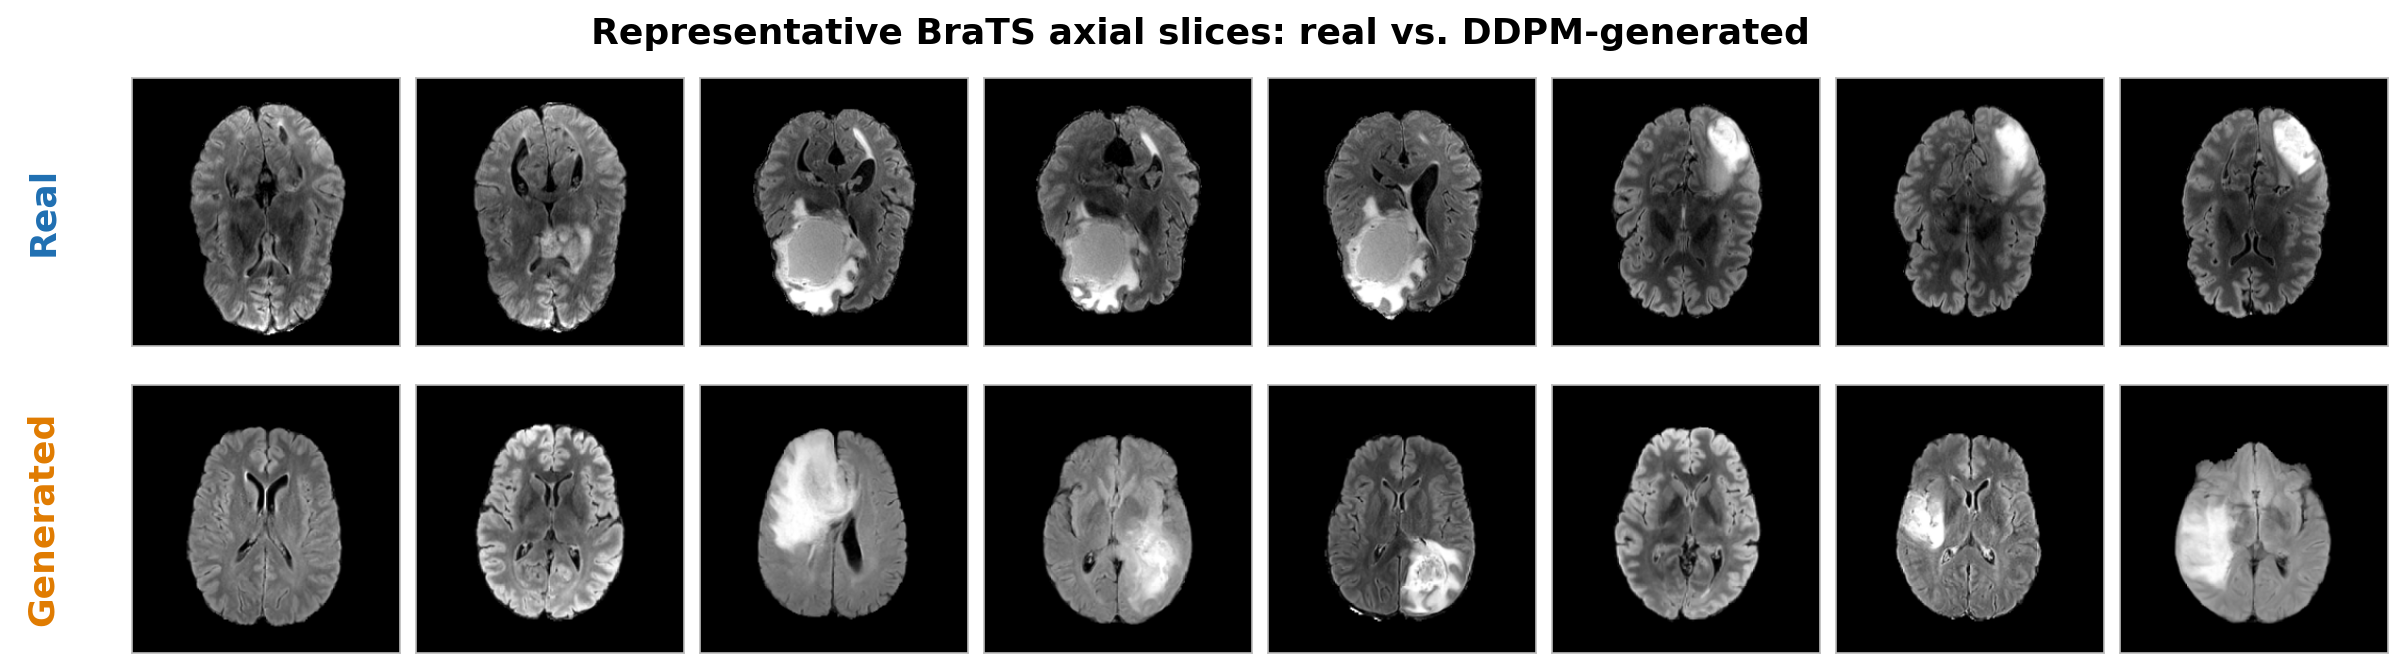
\includegraphics[width=\textwidth]{Images/samples/real_vs_generated.png}
\caption{Representative axial BraTS slices: real (top) and unconditional
DDPM-generated (bottom). Both sets exhibit plausible tissue boundaries,
ventricles, and FLAIR-hyperintense lesions, and are difficult to separate by
visual inspection, which motivates a rigorous distributional metric with
native significance testing rather than a qualitative check. Images are shown
at the $224\times224$ resolution fed to the encoder.}
\label{fig:samples}
\end{figure*}

% ------------------------------------------------------------
\subsection{Baseline Sanity Check: Noise and Blur Robustness}
\label{sec:results_noise}
% ------------------------------------------------------------

A necessary condition for any evaluation metric is monotonic response to
known image degradation.
We inject progressive Gaussian noise
($\sigma \in \{0.0, 0.01, 0.02, 0.05, 0.1, 0.2, 0.5\}$) and Gaussian
blur (radius $r \in \{0, 1, 2, 3, 4\}$ pixels) into the real image set
and compute all nine metrics between the clean reference and the
perturbed set.
FRD is excluded due to incompatibility between the pyradiomics
Laplacian-of-Gaussian filter and BraTS axial image
dimensions~\cite{konz2025frd}.
Table~\ref{tab:noise_spearman} reports Spearman rank correlations
between perturbation level and metric value, together with 95\%
confidence intervals via Fisher $z$-transformation.

\begin{table}[t]
\centering
\caption{%
  Spearman rank correlation $\rho$ between perturbation level and
  metric value ($N = 7$ noise levels; $N = 5$ blur radii).
  $\uparrow$: metric should increase with perturbation.
  $\downarrow$: metric should decrease.
  All $p < 0.001$ except $\alpha$-Precision and $\beta$-Recall
  under blur ($p = 0.005$).
}
\label{tab:noise_spearman}
\setlength{\tabcolsep}{6pt}
\begin{tabular}{lcccc}
\toprule
\multirow{2}{*}{Metric} &
\multirow{2}{*}{Dir.} &
\multicolumn{2}{c}{Spearman $\rho$} \\
\cmidrule(lr){3-4}
& & Noise & Blur \\
\midrule
M3-Score (ours)       & $\uparrow$   & $\mathbf{1.000}$ & $\mathbf{1.000}$ \\
FID (Inception)       & $\uparrow$   & $1.000$          & $1.000$ \\
KID (Inception)       & $\uparrow$   & $1.000$          & $1.000$ \\
SSIM                  & $\downarrow$ & $-1.000$         & $-1.000$ \\
PSNR                  & $\downarrow$ & $-1.000$         & $-1.000$ \\
MS-SSIM               & $\downarrow$ & $-1.000$         & $-1.000$ \\
LPIPS                 & $\uparrow$   & $1.000$          & $1.000$ \\
$\alpha$-Precision    & $\downarrow$ & $-0.982$         & $-0.975$ \\
$\beta$-Recall        & $\downarrow$ & $-0.982$         & $-0.975$ \\
\bottomrule
\end{tabular}
\end{table}

\paragraph{Noise degradation}
At $\sigma = 0$ (clean versus clean), M3 returns exactly $0.0$,
consistent with the unbiased MMD$^2$ estimator whose expectation is
zero under identical distributions.
All nine metrics achieve perfect Spearman correlation ($|\rho| = 1.0$,
$p < 0.001$) under Gaussian noise, confirming that M3 responds
correctly to progressive pixel-level degradation
(Fig.~\ref{fig:noise_robustness} and Fig.~\ref{fig:blur_robustness}).
As noise increases to $\sigma = 0.5$, the fidelity MMD$^2$ rises to
$0.607$, FID to $521.96$, and KID to $0.868$, while SSIM collapses to
$0.031$ and PSNR to $9.29$\,dB (raw unnormalized values; Fig.~\ref{fig:noise_robustness} and Fig.~\ref{fig:blur_robustness} display all metrics normalised to $[0,1]$ for visual comparison).

\paragraph{Blur degradation}
Under Gaussian blur the M3-Score achieves $\rho = 1.000$ ($p < 0.001$),
identical to FID and KID, and the sequence is strictly monotone across
all five radii.
The $\alpha$-Precision metric reveals that blur is substantially more
destructive to manifold membership than noise at comparable image quality.
At blur radius $r = 2$ (PSNR $= 27.88$\,dB), $\alpha$-Precision
collapses to $0.006$: virtually no perturbed images remain within the
real clinical manifold.
At Gaussian noise $\sigma = 0.05$ (PSNR $= 27.96$\,dB, similar
quality), $\alpha$-Precision remains $0.384$.
This confirms that the real BraTS image manifold is defined primarily by
high-frequency texture structure that blur destroys while additive noise
partially preserves.

\begin{figure*}[!t]
\centering
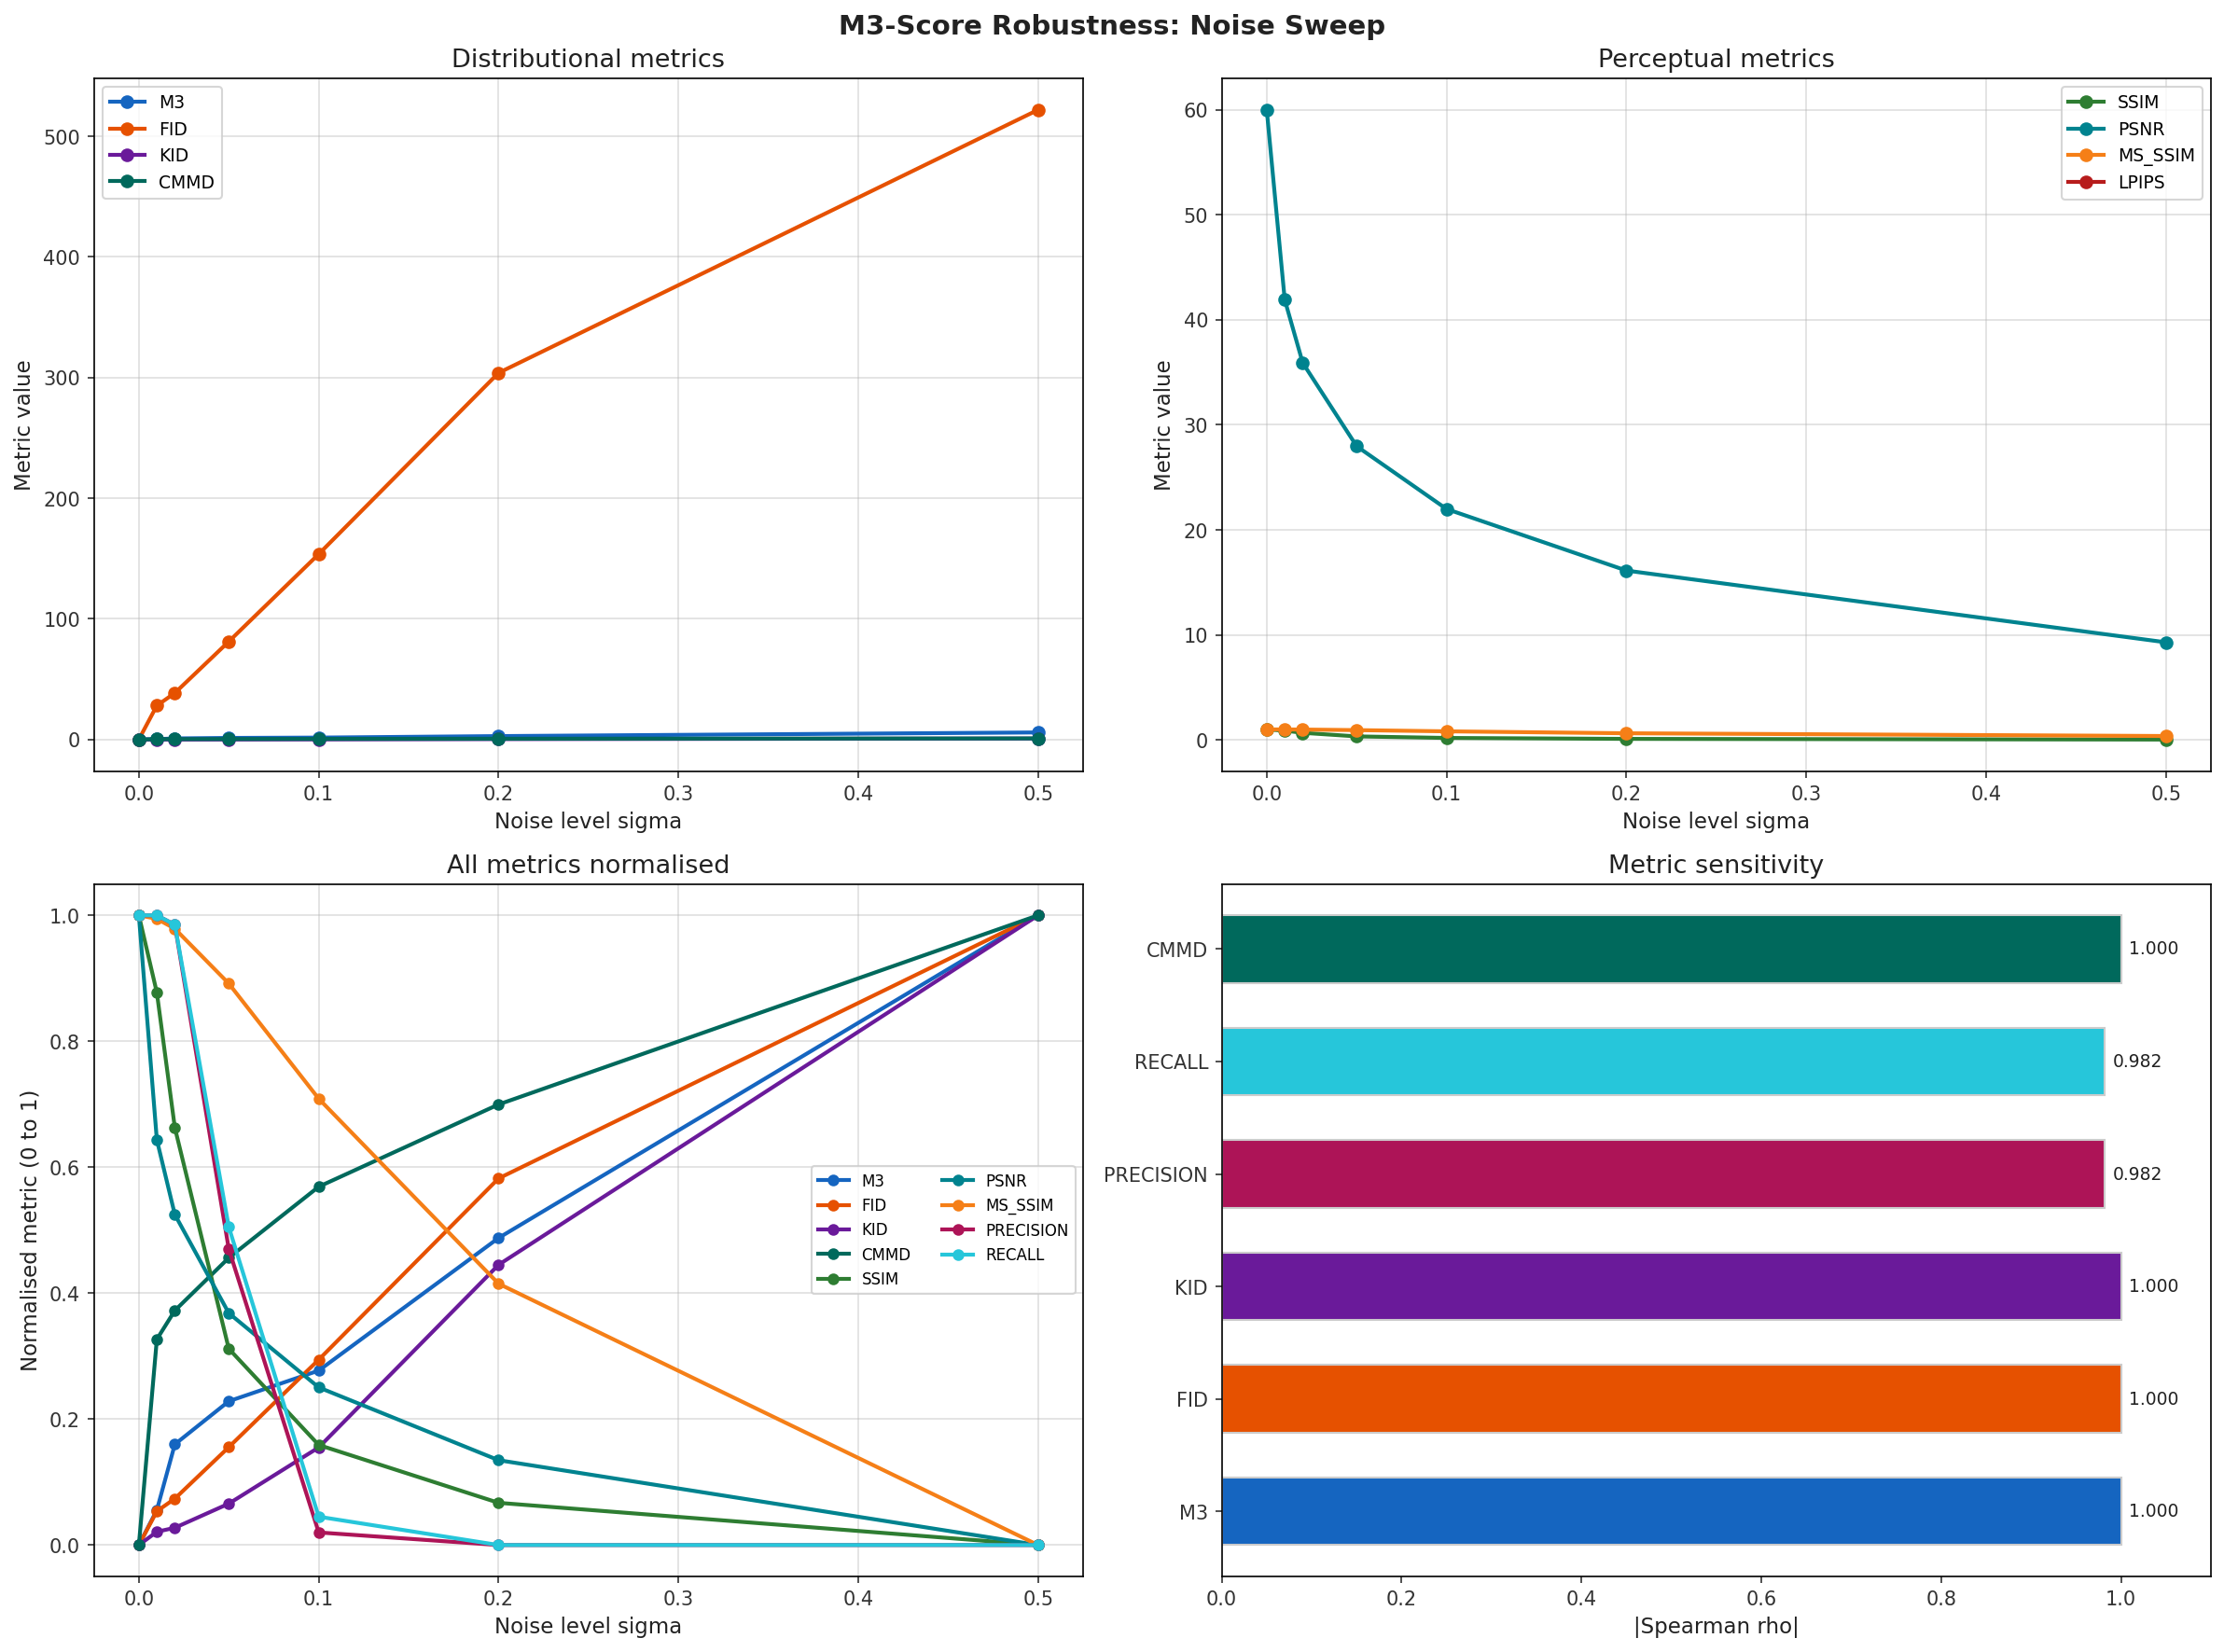
\includegraphics[width=0.85\linewidth]{Images/noise_robustness/noise_robustness.png}
\caption{%
  \textbf{Gaussian noise sweep} ($\sigma \in [0,0.5]$, $N = 200$ BraTS images).
  The composite panel shows four views:
  (a)~distributional metrics (M3/FID/KID) in raw units,
  (b)~perceptual metrics (SSIM/PSNR/MS-SSIM/LPIPS),
  (c)~all metrics normalised to $[0,1]$ for visual comparison, and
  (d)~$|\mathrm{Spearman}\ \rho|$ bar chart.
  All nine metrics achieve $|\rho| = 1.00$ ($p < 0.001$);
  the normalised panel (c) shows M3 and SSIM/PSNR diverge earliest,
  indicating higher sensitivity at low perturbation levels.
  Note: raw metric values cited in text (e.g.\ fidelity MMD$^2 = 0.607$, FID $= 521.96$ at $\sigma = 0.5$)
  correspond to unnormalized panel (a)/(b); panel~(c) shows the same data rescaled.%
}
\label{fig:noise_robustness}
\end{figure*}

\begin{figure*}[!t]
\centering
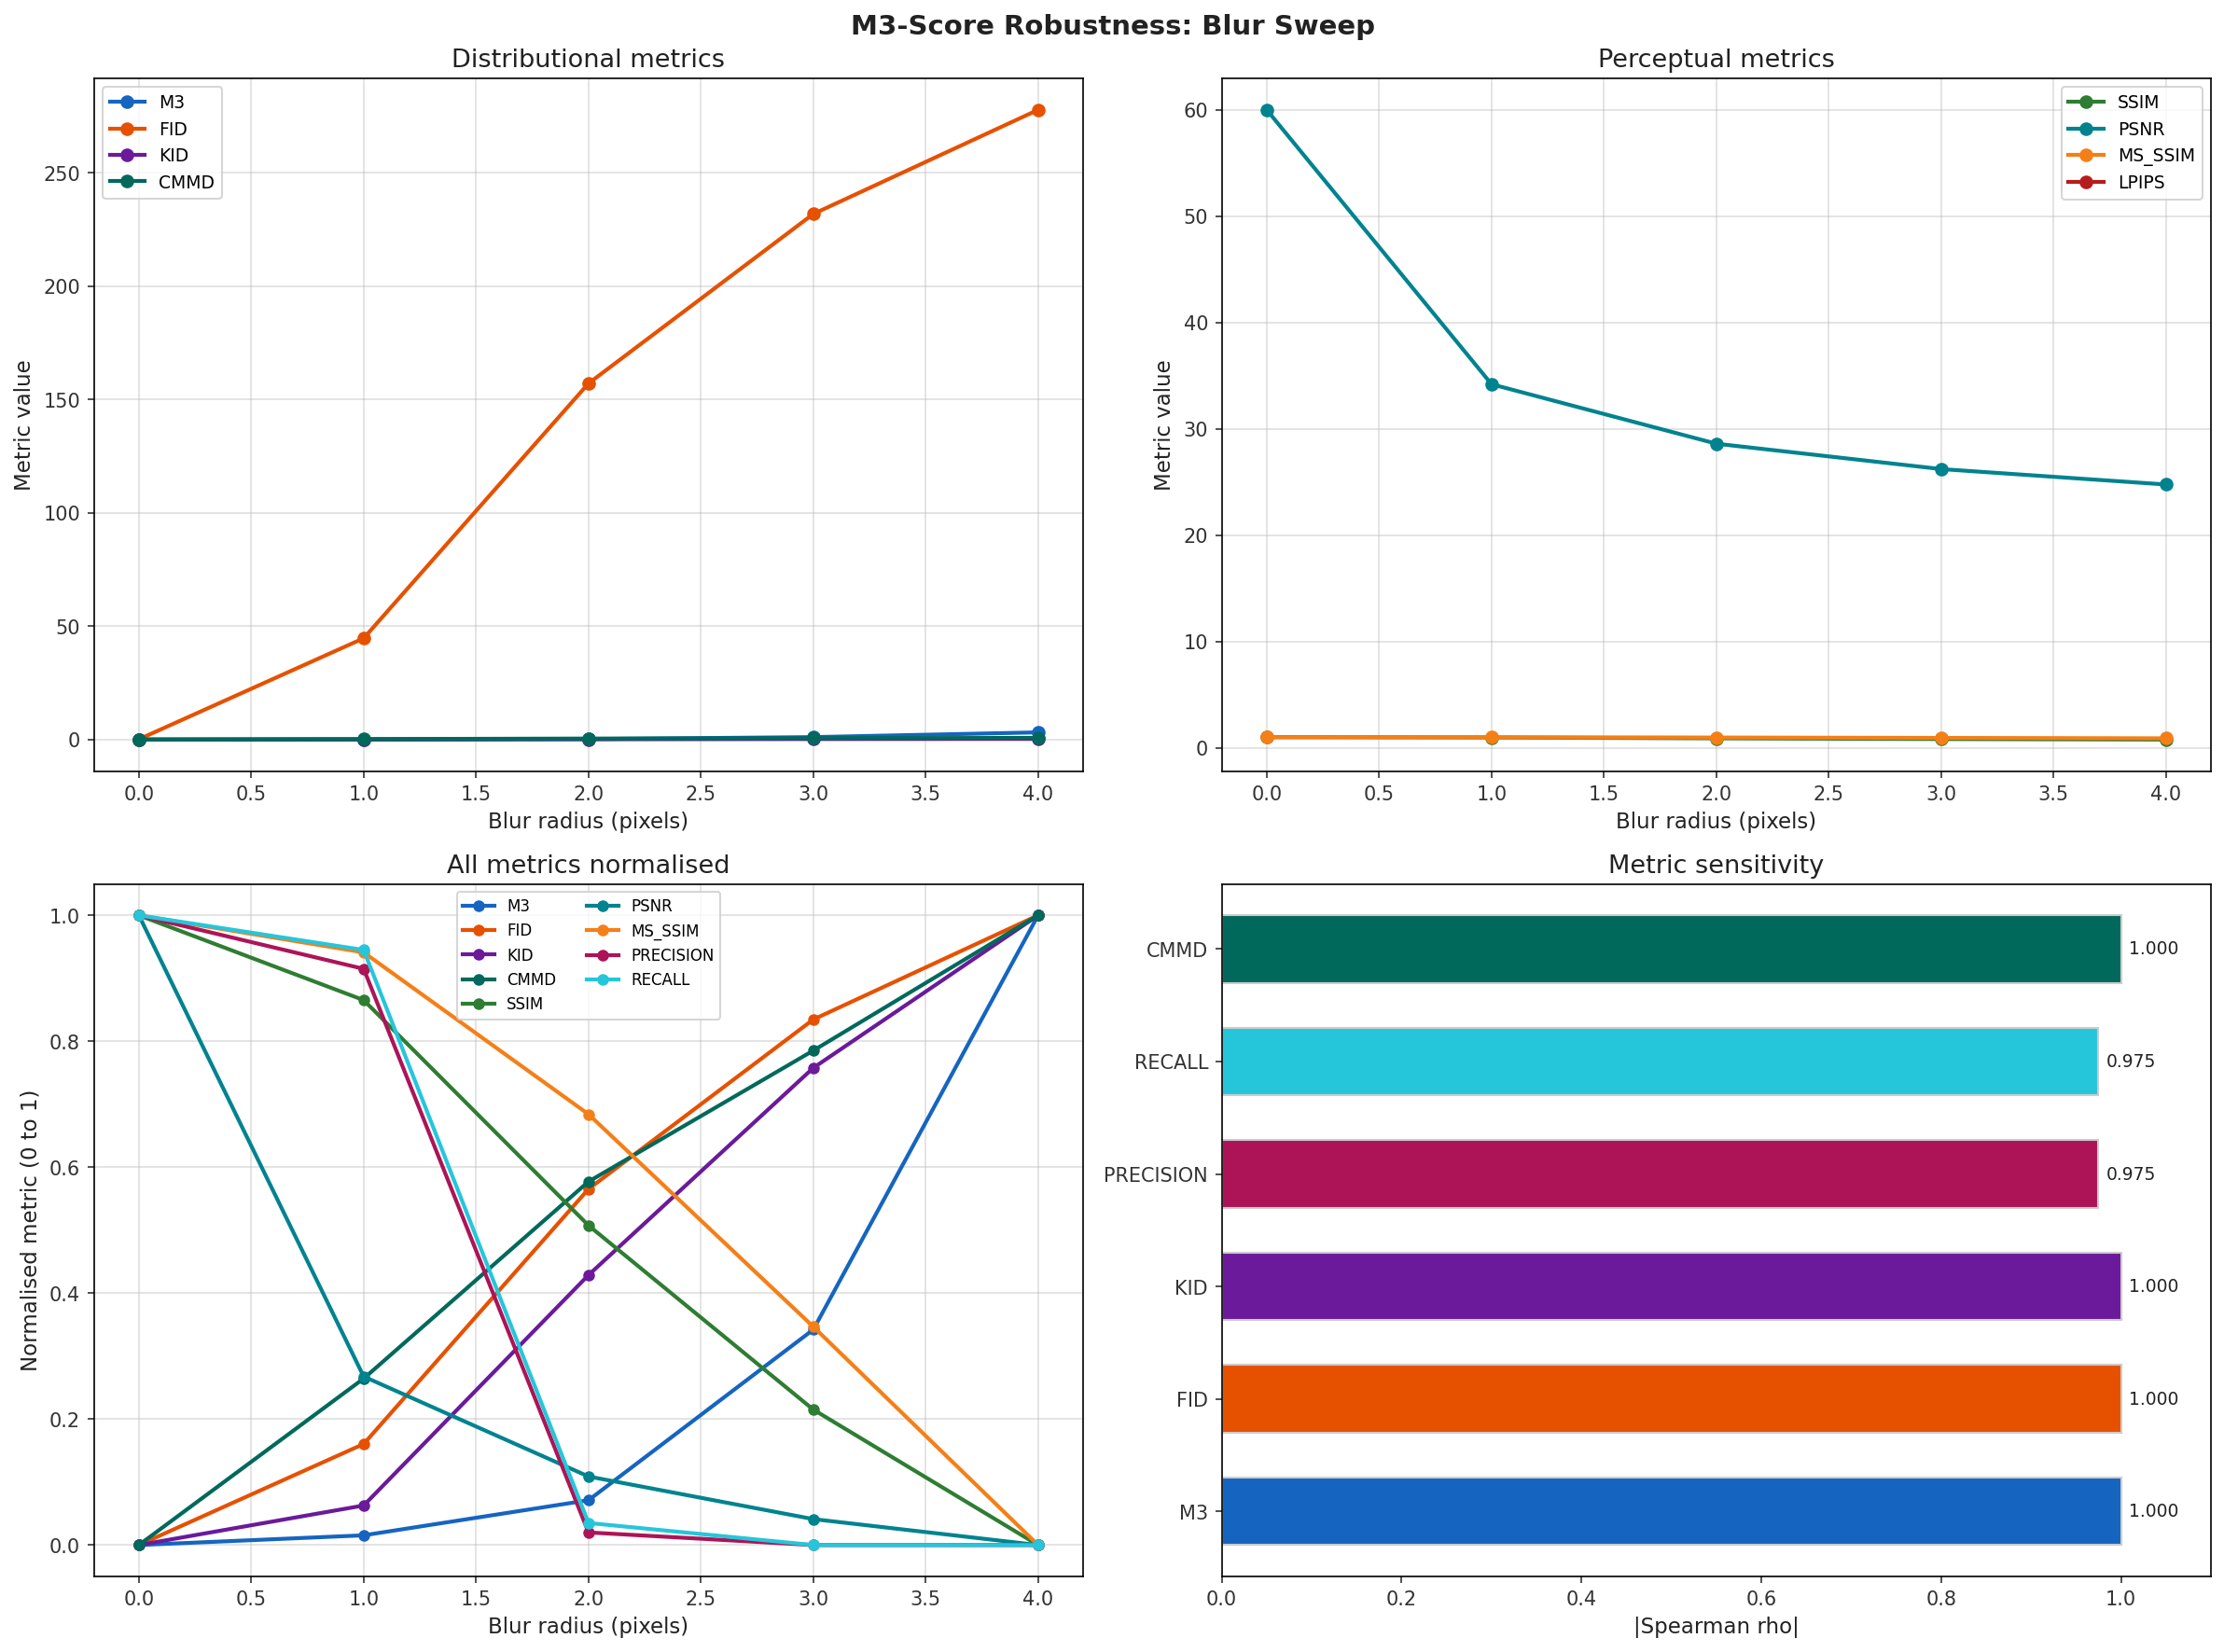
\includegraphics[width=0.85\linewidth]{Images/noise_robustness/blur_robustness.png}
\caption{%
  \textbf{Gaussian blur sweep} ($r \in \{0,1,2,3,4\}$ pixels, $N = 200$ BraTS images).
  The composite panel shows four views:
  (a)~distributional metrics (M3/FID/KID) in raw units,
  (b)~perceptual metrics (SSIM/PSNR/MS-SSIM/LPIPS),
  (c)~all metrics normalised to $[0,1]$ for visual comparison, and
  (d)~$|\mathrm{Spearman}\ \rho|$ bar chart.
  M3-Score achieves $\rho = 1.000$ ($p < 0.001$).
  $\alpha$-Precision collapses to $0.006$ by $r = 2$, while distributional metrics
  remain monotonic, revealing that the real BraTS manifold is defined by
  high-frequency texture structure that Gaussian blur selectively destroys.%
}
\label{fig:blur_robustness}
\end{figure*}

% ------------------------------------------------------------
\subsection{Unsupervised Anomaly Detection and OOD Correlation}
\label{sec:results_ood}
% ------------------------------------------------------------

A central claim of the M3-Score is that its fidelity axis identifies
clinically anomalous generated images without requiring explicit anomaly
labels.
We test this by fitting an Isolation Forest~\cite{liu2008isolation} on
embeddings of the $500$ real images and scoring each of the
$500$ generated images independently of M3.
The fidelity axis uses the a-priori layer $\ell_{\text{fid}} = 12$
(Section~\ref{sec:method_axes}); no adaptive weighting is involved.

\paragraph{OOD rate}
With contamination threshold $0.05$, $16.0\%$ of generated images
($80$ of $500$) are flagged as out-of-distribution.
The mean anomaly score of generated images ($-0.020$) is systematically
higher than that of real images ($-0.047$), confirming that the
generated distribution occupies lower-probability regions of the real
clinical manifold.

\paragraph{Per-image score correlation}
Table~\ref{tab:ood_spearman} reports Spearman correlations between the
Isolation Forest anomaly score and three per-image distance measures.

\begin{table}[t]
\centering
\caption{%
  Spearman correlation between per-image Isolation Forest anomaly score
  and per-image distance measures ($N = 500$ generated images).
  95\% CIs via Fisher $z$-transformation.
}
\label{tab:ood_spearman}
\begin{tabular}{lccc}
\toprule
Distance measure & $\rho$ & $p$ & 95\% CI \\
\midrule
M3-Score (RadioDINO, L2-norm) & $\mathbf{+0.238}$ & $7.5 \times 10^{-8}$ & $[0.153,\;0.319]$ \\
FID proxy (InceptionV3)     & $+0.211$          & $2.0 \times 10^{-6}$ & $[0.126,\;0.293]$ \\
Pixel MSE                   & $-0.199$          & $7.5 \times 10^{-6}$ & $[-0.282,\;-0.113]$ \\
\bottomrule
\end{tabular}
\end{table}

M3 per-image scores show the highest point correlation with the independent
anomaly detector ($\rho = +0.238$, $p = 7.5 \times 10^{-8}$), slightly above
the FID proxy ($\rho = +0.211$) despite using a completely different backbone
and distance measure. However, the two $95\%$ CIs overlap
($[0.153,0.319]$ vs.\ $[0.126,0.293]$), so this per-image ranking difference is
\emph{not} statistically significant: at the per-image level M3 and the FID
proxy are comparable, and M3's advantage over FID is established at the
\emph{distributional} level instead (ROC-AUC and the permutation test,
Section~\ref{sec:results_ood}), not in per-image anomaly ranking.
Pixel MSE exhibits a significant \emph{negative} correlation
($\rho = -0.199$), confirming the well-documented failure of pixel-space
distances to capture clinical anomaly: an image can be pixel-similar to
the real mean while being semantically implausible in clinical terms
(Fig.~\ref{fig:ood}\,(b)).

\paragraph{Binary distributional separation}
To formally quantify whether RadioDINO or InceptionV3 features provide
better separation between real and generated images, we treat the
centroid-L2 distance as a binary classifier score (real $= 0$,
generated $= 1$) and compute ROC-AUC and PR-AUC for both backbones.
Tables~\ref{tab:ood_metric} and~\ref{tab:ood_sweep} report the results.

\begin{table}[t]
\centering
\caption{%
  \textbf{Metric-backbone comparison} at the canonical $N = 500$: OOD ROC-AUC
  (BraTS real vs.\ DDPM-generated, centroid-$L_2$ score). The M3 fidelity
  backbone is compared against the backbones that underlie FID and CMMD.
}
\label{tab:ood_metric}
\begin{tabular}{lc}
\toprule
Metric (backbone) & OOD ROC-AUC ($N{=}500$) \\
\midrule
\textbf{M3 (RadioDINO-s16, ours)} & $\mathbf{0.976}$ \\
FID (InceptionV3)                 & $0.809$ \\
CMMD (CLIP ViT-L/14)              & $0.659$ \\
\bottomrule
\end{tabular}
\end{table}

\begin{table}[t]
\centering
\caption{%
  \textbf{Backbone selection screen} for the M3 fidelity axis: OOD ROC-AUC
  across candidate medical/general encoders (BraTS real vs.\ DDPM-generated,
  $N = 100$). RadioDINO-s16 is selected for all other experiments; it also
  leads at $N = 500$ (Table~\ref{tab:ood_metric}), so the choice is not an
  artifact of the screening sample size.
}
\label{tab:ood_sweep}
\begin{tabular}{lc}
\toprule
Candidate backbone & OOD ROC-AUC ($N{=}100$) \\
\midrule
\textbf{RadioDINO-s16 (ours)}   & $\mathbf{0.995}$ \\
DINOv2-base (ViT-B/14)          & $0.968$ \\
RadImageNet-ResNet50            & $0.954$ \\
PubMed-CLIP                     & $0.921$ \\
Microsoft rad-dino (ViT-B/14)   & $0.913$ \\
\bottomrule
\end{tabular}
\end{table}

The RadioDINO-s16 fidelity axis achieves ROC-AUC $= 0.976$ at $N = 500$
versus $0.809$ for InceptionV3 (the FID backbone) and $0.659$ for CLIP
(the CMMD backbone), a $+20.6\%$ and $+48.1\%$ relative margin
respectively (Fig.~\ref{fig:ood}\,(c)). The $N = 100$ six-backbone selection
screen (Table~\ref{tab:ood_sweep}) confirms the choice: RadioDINO-s16
($0.995$) leads the larger Microsoft rad-dino ViT-B/14 ($0.913$) and
generic DINOv2 ($0.968$). Notably, the most ``distinctive'' backbone by
inter-layer CKA (rad-dino, L1$\leftrightarrow$L12 CKA $= 0.203$) is the
\emph{worst} OOD discriminator, so layer distinctiveness does not predict
discriminative power; we select by OOD-AUC, not by CKA structure.

\paragraph{CMMD structural failure on medical OOD ordering}
The most consequential comparison is not the aggregate AUC but a specific
ordering failure. We evaluate three tiers against BraTS real ($N = 500$, with
bootstrap $95\%$ CIs over $500$ resamples): a same-domain DDPM generator, a
weaker same-domain (WDM-3D) generator, and a full cross-modality shift to
chest/lung CT (LIDC). CMMD here follows the standard protocol of
Jayasumana~\textit{et al.}~\cite{jayasumana2024cmmd}: OpenAI CLIP
ViT-L/14 image features and an unbiased Gaussian-RBF MMD$^2$ with the
median-heuristic bandwidth computed on the pooled real-plus-generated sample,
so the inversion below cannot be attributed to a non-standard estimator or
bandwidth. The correct order is DDPM $<$ WDM-3D $<$ CT, since a
different modality should be the most distant; the three tiers are illustrated
in Fig.~\ref{fig:tiers}. The M3 fidelity axis recovers
this order with non-overlapping CIs
($0.153 < 0.248 < 0.457$; Table~\ref{tab:cmmd_fail}). CMMD, however,
\emph{inverts} the last two tiers: it assigns the cross-modality CT
($0.699\,[0.686,0.715]$) a \emph{smaller} distance than the weak same-modality
MRI generator ($0.738\,[0.723,0.758]$), ranking lung CT as closer to brain
MRI than a poor brain-MRI generator. The paired difference
$\Delta_{\mathrm{CT}-\mathrm{MRI}} = -0.039\,[-0.059,-0.021]$ excludes zero,
so this is a statistically significant rank inversion, not sampling noise; the
corresponding M3 difference is $+0.210\,[+0.198,+0.220]$. Crucially, FID
(InceptionV3) also orders the tiers correctly ($68.8 < 180.6 < 317.4$), so the
failure is specific to \emph{CLIP} features rather than to natural-image
backbones in general: CLIP does not encode the radiology modality boundary
that a radiology-trained backbone, and even InceptionV3, does. (These values
supersede an earlier draft that reported the CMMD tiers as $0.674$ vs.\ $0.663$
with $\Delta = 0.011$; under bootstrap CIs the effect is a significant
inversion, which is a stronger form of the same structural limitation.)

\begin{figure*}[!t]
\centering
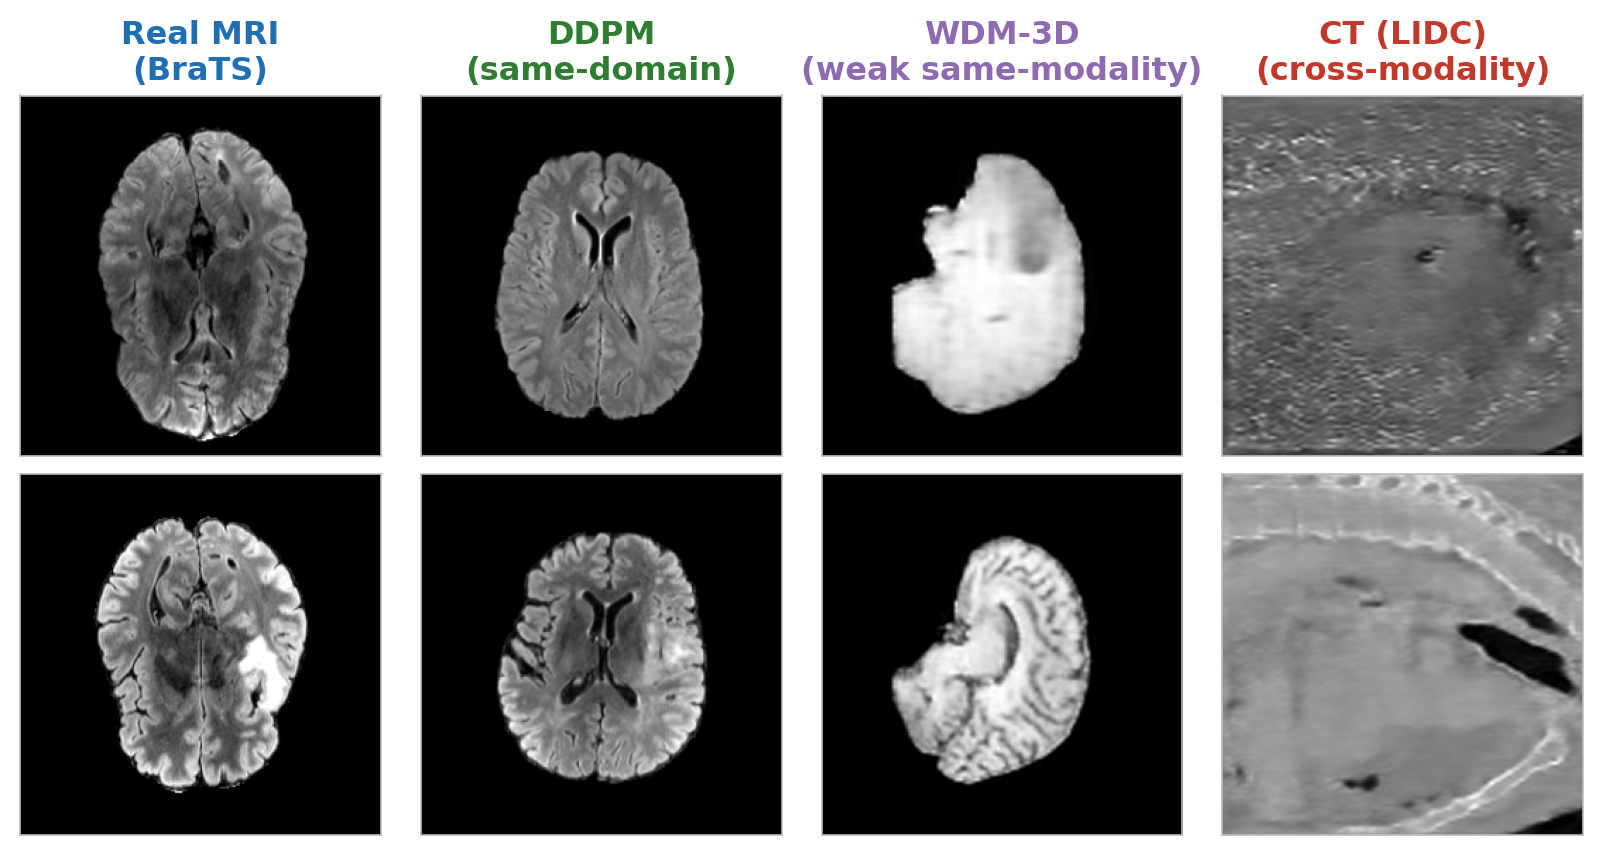
\includegraphics[width=\textwidth]{Images/samples/cross_modality_tiers.png}
\caption{The three tiers evaluated against real BraTS MRI. From left: real MRI;
a same-domain DDPM generator; a weaker same-modality WDM-3D generator (visibly
lower-quality but still brain MRI); and a cross-modality LIDC chest CT scan,
which is a different modality and anatomy. A faithful metric should rank the CT
as the most distant from real brain MRI. M3 and FID do; CMMD inverts the last
two, ranking the CT (right) as closer to real MRI than the weak WDM-3D brain
generator (Table~\ref{tab:cmmd_fail}).}
\label{fig:tiers}
\end{figure*}

\begin{table}[t]
\centering
\caption{%
  Cross-tier separation from BraTS real ($N = 500$; bootstrap $95\%$ CIs for
  M3 and CMMD over $500$ resamples). Higher $=$ more distant, so the correct
  order is DDPM $<$ WDM-3D $<$ CT. M3 and FID order the tiers correctly; CMMD
  \emph{inverts} the last two, ranking cross-modality CT as closer than the
  weak MRI generator ($\Delta_{\mathrm{CT}-\mathrm{MRI}} < 0$, CI excludes
  zero). FID values are point estimates (InceptionV3).
}
\label{tab:cmmd_fail}
\setlength{\tabcolsep}{4pt}
\resizebox{\columnwidth}{!}{%
\begin{tabular}{lccc}
\toprule
Comparison vs.\ BraTS real & M3 (fid.) [95\% CI] & FID & CMMD [95\% CI] \\
\midrule
DDPM (same-domain)           & $0.153\,[0.146,0.162]$ & $68.8$  & $0.133\,[0.129,0.144]$ \\
WDM-3D (weak same-domain)    & $0.248\,[0.243,0.257]$ & $180.6$ & $0.738\,[0.723,0.758]$ \\
LIDC CT (cross-modality OOD) & $\mathbf{0.457}\,[0.449,0.472]$ & $317.4$ & $0.699\,[0.686,0.715]$ \\
\midrule
CT $-$ WDM-3D\ \ $\Delta$    & $\mathbf{+0.210}\,[+0.198,+0.220]$ & $+136.8$ & $-0.039\,[-0.059,-0.021]$ \\
\bottomrule
\end{tabular}}
\end{table}

\paragraph{Domain-ontology ordering (honest caveat)}
Across five test sets ordered by intuitive OOD severity, FID and KID
achieve Kendall $\tau = 1.000$ while M3 achieves $\tau = 0.800$
($p = 0.083$). The single inversion is that M3 ranks retinal fundus images
as \emph{further} from brain MRI than chest CT. This is not an error: under
a radiology-domain ontology, CT and MRI are neighbours and fundus is
out-of-domain, which RadioDINO correctly reflects. It does, however, mean
M3 should not be read as a universal visual-distance metric, and we restrict
its claims to the radiology domain accordingly.

\begin{figure*}[!t]
\centering

\begin{subfigure}[t]{0.48\textwidth}
    \centering
    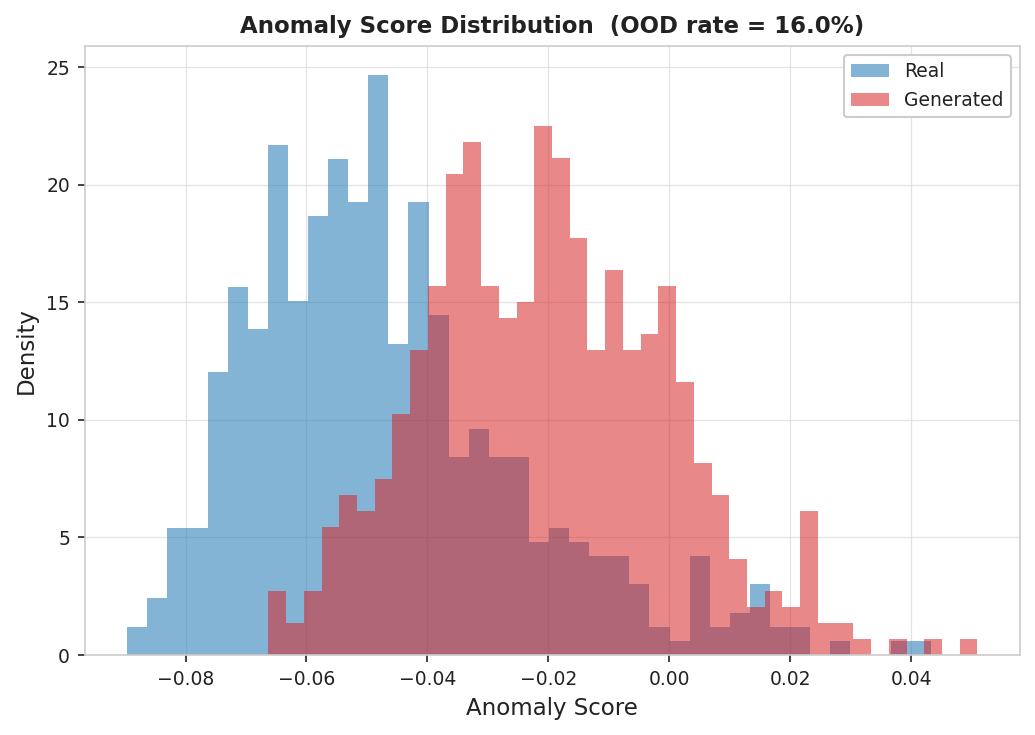
\includegraphics[width=\linewidth]{Images/OOD/ood_distributions.png}
    \caption{Score distributions. Real (blue) and generated (orange)
    Isolation Forest anomaly scores form distinct populations; $16\%$
    of generated images exceed the OOD threshold (dashed).}
    \label{fig:ood_dist}
\end{subfigure}
\hfill
\begin{subfigure}[t]{0.48\textwidth}
    \centering
    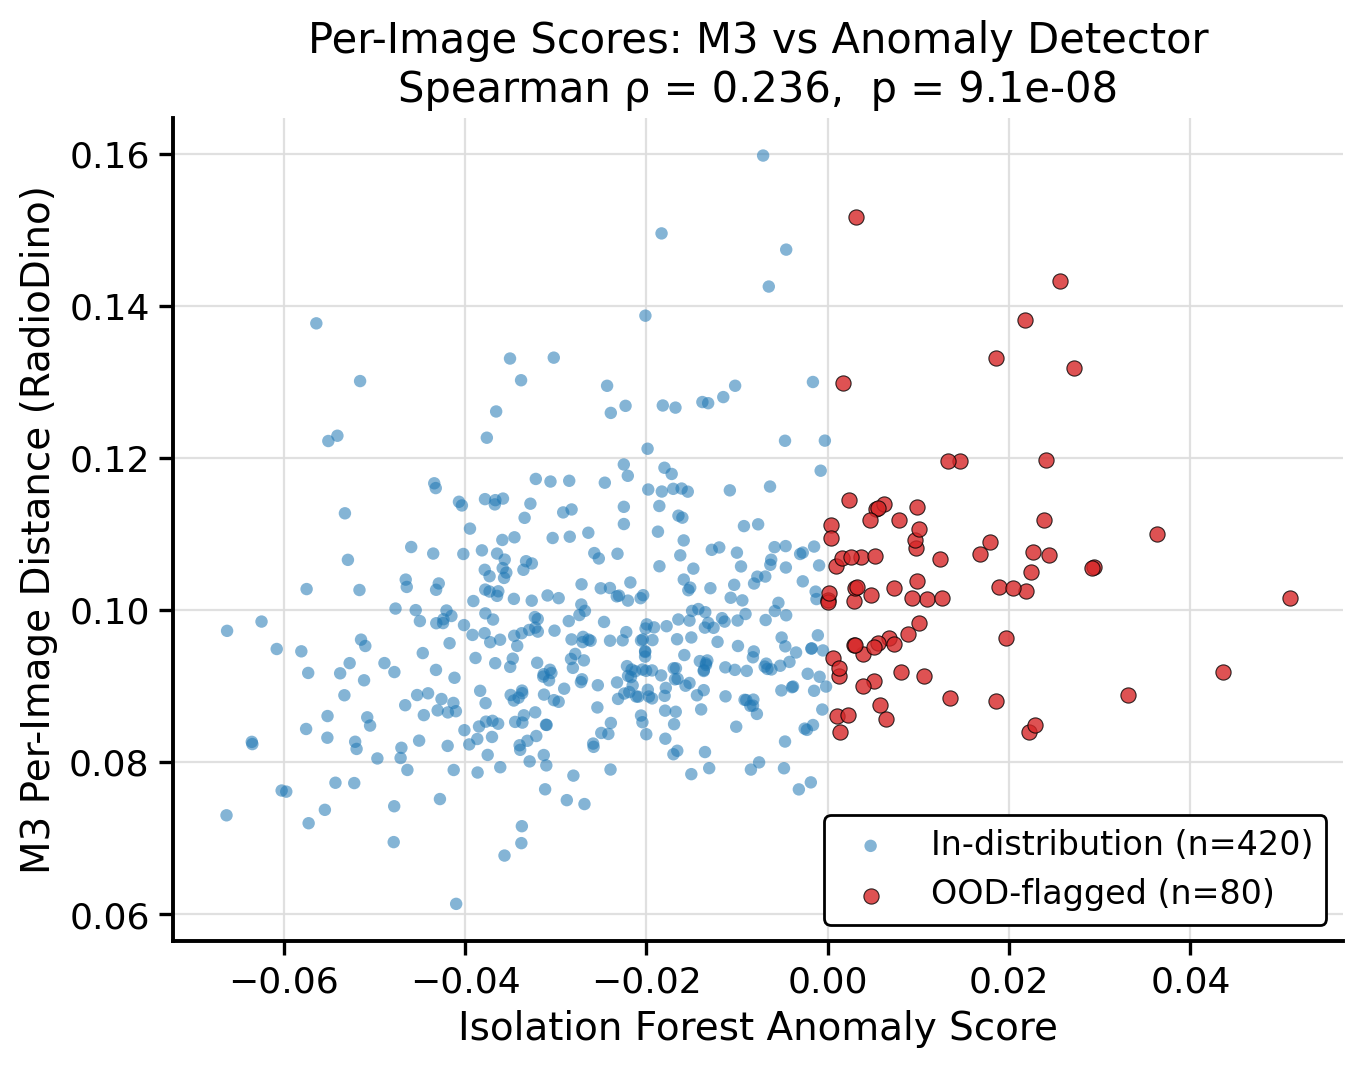
\includegraphics[width=\linewidth]{Images/OOD/ood_comparison_scatter.png}
    \caption{Per-image score scatter. M3 per-image distances (y-axis)
    versus Isolation Forest anomaly score (x-axis) for $N = 500$
    generated images; red markers are OOD-flagged images.
    Spearman $\rho = +0.238$, $p = 7.5 \times 10^{-8}$.}
    \label{fig:ood_scatter}
\end{subfigure}

\vspace{0.5em}

\begin{subfigure}[t]{0.62\textwidth}
    \centering
    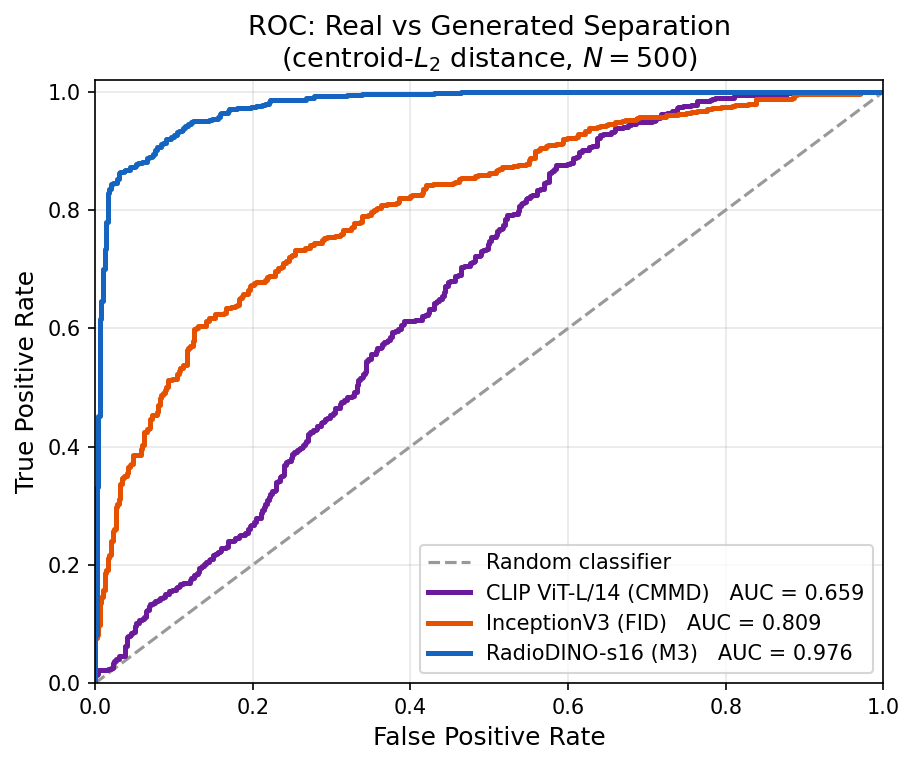
\includegraphics[width=\linewidth]{Images/OOD/ood_roc_auc.png}
    \caption{ROC curves. RadioDINO-s16 features (M3 backbone,
    AUC $= 0.976$) substantially outperform InceptionV3
    features (FID backbone, AUC $= 0.809$) and CLIP
    (CMMD backbone, AUC $= 0.659$) in separating
    real from generated images without anomaly labels.}
    \label{fig:ood_roc}
\end{subfigure}

\caption{Unsupervised anomaly detection results ($N = 500$ per class).
(a) Score distributions show clear separation between real and generated
populations. (b) M3 per-image scores correlate significantly with the
independent Isolation Forest detector. (c) RadioDINO-s16 features achieve
ROC-AUC $0.976$, a $20.6\%$ improvement over InceptionV3 ($0.809$) and a
$48\%$ improvement over CLIP ($0.659$).}

\label{fig:ood}

\end{figure*}
\subsection{Three-Axis Validation}
\label{sec:results_axes}
% ------------------------------------------------------------

We validate the memorization and coverage axes by injecting the specific
failure each is designed to detect and checking that the corresponding
axis, and only that axis, responds. Features are read from the a-priori
layers $\ell_{\text{mem}} = 9$ and $\ell_{\text{cov}} = 4$
(Section~\ref{sec:method_axes}); $N = 150$ BraTS real and DDPM-generated
images.

\paragraph{Memorization axis (validated)}
We replace a known fraction of generated images with near-duplicates of
real images (Gaussian jitter, $\sigma = 5\times10^{-4}$) at injection
rates $\{0.0, 0.1, 0.2, 0.3, 0.5\}$. The L9 memorization rate recovers the
injection rate \emph{exactly} ($0.00, 0.10, 0.20, 0.30, 0.50$;
Table~\ref{tab:axes}), confirming the axis flags near-duplicates at the
intended depth. As expected, the fidelity MMD$^2$ at L12 simultaneously
falls (from $0.187$ to $0.043$), because injecting genuine real images into
the generated set also moves the generated distribution toward the real one;
the two axes are therefore correlated under this perturbation rather than
orthogonal, which we report rather than obscure.

\begin{table}[t]
\centering
\caption{%
  Memorization-axis injection test ($N = 150$). The L9 memorization rate
  recovers the injected near-duplicate fraction exactly; L12 fidelity also
  responds because injected real images shift the generated distribution.
}
\label{tab:axes}
\begin{tabular}{lccc}
\toprule
Injection rate & Mem.\ rate (L9) & Fidelity MMD$^2$ (L12) & Coverage recall (L4) \\
\midrule
$0.0$ & $0.00$ & $0.187$ & $0.18$ \\
$0.1$ & $0.10$ & $0.150$ & $0.89$ \\
$0.2$ & $0.20$ & $0.116$ & $0.93$ \\
$0.3$ & $0.30$ & $0.090$ & $1.00$ \\
$0.5$ & $0.50$ & $0.043$ & $0.99$ \\
\bottomrule
\end{tabular}
\end{table}

\paragraph{Coverage axis (honest negative)}
Probing the coverage axis with mode-drop (truncating the generated set by
$\{0, 10, 20, 30, 50\}\%$) does \emph{not} produce a monotone decrease in
L4 recall; recall instead drifts upward ($0.18 \to 0.28$) as the generated
set shrinks. The mechanism is well understood: with fewer generated points,
each point's $k$-NN radius inflates, the generated manifold balls expand,
and they cover more real points despite reduced diversity. This is a known
instability of $k$-NN precision/recall at small $N$~\cite{kynkaanniemi2019pr,naeem2020dc}.
We therefore report the coverage axis as a diagnostic under active
development, not a validated claim, and recommend it only with
$N \gtrsim 500$ and semantically clustered mode-drop. Precision is
identically $0.0$ in our setting, consistent with the OOD result that
generated points lie outside the real $k$-NN manifold at this checkpoint.

% ------------------------------------------------------------
\subsection{Generation-Quality Ladder}
\label{sec:results_ladder}
% ------------------------------------------------------------

A metric must order images by known generation quality. We construct a
quality ladder over the number of DDPM denoising steps
$T \in \{10, 20, 50, 100, 1000\}$ (more steps $=$ higher quality) from a
fixed checkpoint, and compute the fidelity axis, FID, and CMMD against the
real set. All three metrics are monotone in the correct direction
(Table~\ref{tab:ladder}): each decreases as $T$ rises. Most of the
discriminative signal lies between $T = 100$ and $T = 1000$; the metrics
barely separate $T = 10$ from $T = 100$, a limitation of the
noise-proxy construction we used to generate the ladder under compute
constraints. M3 holds no unique advantage in ordering here. Its advantage
is the native significance test (below), not monotonicity, which FID and
KID also satisfy.

\begin{table}[t]
\centering
\caption{%
  Generation-quality ladder over DDPM denoising steps $T$ ($N = 150$).
  All metrics decrease monotonically as quality improves (Spearman
  $\rho = -1.0$ for each).
}
\label{tab:ladder}
\begin{tabular}{lccc}
\toprule
Denoising steps $T$ & M3 (fid.) & FID & CMMD \\
\midrule
$10$   & $0.616$ & $358.8$ & $0.469$ \\
$20$   & $0.614$ & $357.5$ & $0.467$ \\
$50$   & $0.608$ & $353.8$ & $0.462$ \\
$100$  & $0.598$ & $347.6$ & $0.452$ \\
$1000$ & $\mathbf{0.187}$ & $\mathbf{132.4}$ & $\mathbf{0.112}$ \\
\bottomrule
\end{tabular}
\end{table}

% ------------------------------------------------------------
\subsection{Lesion-Specificity with Real Expert Masks}
\label{sec:results_masking}
% ------------------------------------------------------------

A radiology-trained backbone should, in principle, respond more strongly to
degradation of the diagnostically relevant region than to equal-area
degradation of healthy tissue, a property natural-image backbones need not
possess. We test this directly using the \emph{real} expert
FLAIR-abnormality segmentations of the lower-grade-glioma (LGG) dataset
of Buda et al.~\cite{buda2019association} ($600$ image--mask pairs),
replacing the intensity-threshold proxy masks of earlier drafts.

The test is a within-image, area-matched contrast. For each image we perturb
(i) the annotated tumour region [\textsc{lesion}] versus (ii) an equal-area,
equal-shape region relocated to healthy tissue [\textsc{control}]. We use two
independent control constructions: a \emph{mirror} control (the tumour mask
reflected to the contralateral hemisphere) and a \emph{texture-matched}
control (the tumour mask translated to the healthy-brain location whose local
gradient energy best matches the tumour's). Cases where a control lands off
brain or on tumour are discarded, so lesion and control areas are identical by
construction. We report the specificity ratio
$\rho = \Delta_{\textsc{lesion}}/\Delta_{\textsc{control}}$, where $\Delta$ is
the distributional shift (real vs.\ perturbed) induced by the perturbation;
$\rho > 1$ means the metric reacts more to tumour damage than to equal-area
healthy damage. The baseline is KID (unbiased Inception-MMD), which is valid at
small $N$ and lies in the \emph{same estimator family} as M3, so the backbone
is the only difference between the two. Figure~\ref{fig:lesion_example}
illustrates the two conditions.

\begin{figure*}[!t]
\centering
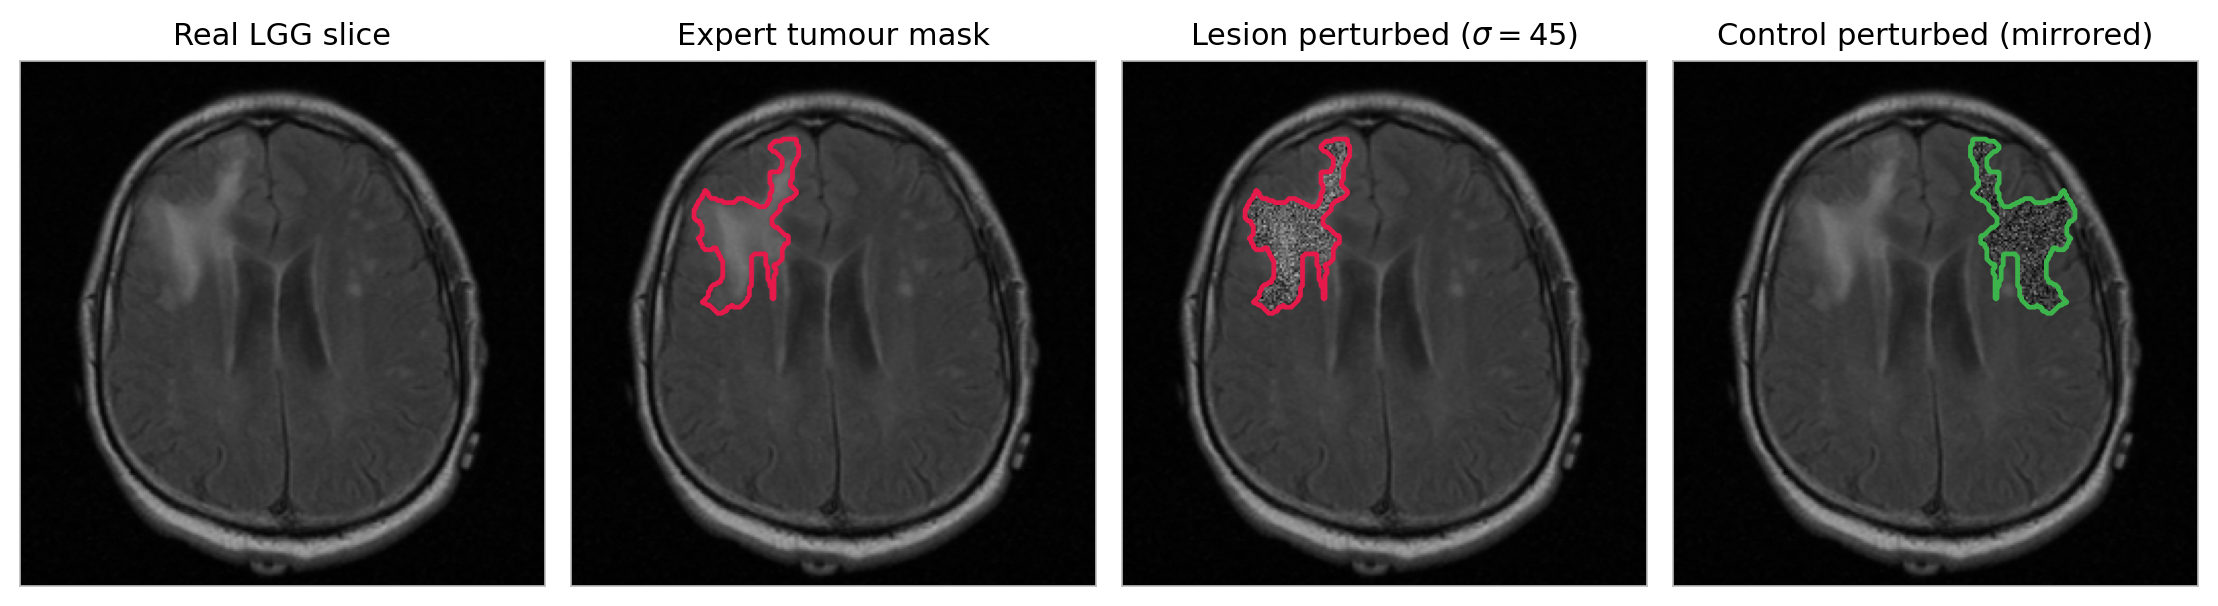
\includegraphics[width=\textwidth]{Images/lesion_specificity/lesion_example.png}
\caption{The area-matched lesion-specificity test on a real LGG slice. From
left: the raw slice; the expert FLAIR-abnormality mask (red); the
\textsc{lesion} condition (region-local Gaussian noise, $\sigma = 45$, inside
the tumour, red); and the \textsc{control} condition (the same noise inside the
mirrored, equal-area contralateral region, green). Lesion and control regions
are identical in shape and area, so any difference in metric response is
attributable to \emph{where} the perturbation is applied, not to how much of the
image is changed.}
\label{fig:lesion_example}
\end{figure*}

Two regimes emerge. Under \emph{gross erasure} (zeroing the region) neither M3
nor KID is lesion-specific ($\rho \approx 1.1$--$1.3$ for both): the black-hole
signal dominates and swamps any semantic difference, consistent with, and
explaining, the artefact-invariance of M3 discussed below. Under \emph{subtle}
region-local Gaussian noise, however, M3 is lesion-selective while the
Inception baseline is not. Figure~\ref{fig:lgg_sweep} traces $\rho$ against
noise strength $\sigma$: in the measurable regime ($\sigma \ge 45$; below this
the L12 MMD$^2$ underflows to zero at $N=200$ and the ratio is undefined) M3
attains $\rho = 1.4$--$1.8$ against \emph{both} controls, which agree to within
$0.1$, whereas KID stays flat at $\rho \approx 1.05$. Because both metrics score
the \emph{identical} perturbed images, and because the mirror control's mean
gradient energy matches the lesion's to within $4\%$, the selectivity is
attributable to the radiology backbone rather than to pixel magnitude or
texture complexity. The effect decays as $\sigma$ grows (extrapolating toward
the $\rho\approx1.1$ of gross erasure), so it is correctly scoped as
selectivity to \emph{subtle} diagnostic-region degradation, not a universal
pathology-sensitivity advantage. As no LGG generator was available, this is a
metric-sensitivity test on real images under controlled perturbations, not a
generator-quality result.

\begin{figure}[t]
\centering

\includegraphics[width=0.95\linewidth]{Images/lesion_specificity/lgg_noise_sweep.png}
\caption{%
  Lesion/healthy specificity ratio $\rho$ versus region-local noise $\sigma$ on
  real LGG expert masks ($N=200$). M3 (red/orange) is lesion-selective
  ($\rho=1.4$--$1.8$) against both the mirror and texture-matched controls,
  which nearly coincide; the Inception-MMD baseline (grey) stays at
  $\rho\approx1.05$. Bands are bootstrap $95\%$ CIs. Points below the M3
  detection floor ($\sigma<45$) are omitted.}
\label{fig:lgg_sweep}
\end{figure}

For completeness we retain the earlier proxy-mask experiment as secondary
evidence of the \emph{opposite} property, that FID and CMMD are driven by
low-level masking artefacts. Across three conditions ($N=200$;
Table~\ref{tab:masking}) with a $64{\times}64$ centre square mask on BraTS,
masking the tumour region in real images (condition~B) moves them \emph{closer}
to the tumour-free generated distribution in RadioDINO space (the M3 fidelity
axis falls by $54.4\%$), whereas FID \emph{increases} by $101.4\%$ and CMMD by
$191.7\%$. InceptionV3 and CLIP features are thus highly sensitive to the
black-square artefact itself, while M3 is comparatively \emph{invariant} to it.
Together with the LGG result, the picture is one of \emph{specificity}:
RadioDINO features track clinically meaningful change (subtle lesion
degradation) rather than pixel-level artefacts that inflate FID and CMMD.
(These BraTS masks are intensity-threshold FLAIR proxies, not ground truth, and
are reported as a conservative supporting result only.)

\begin{table}[t]
\centering
\caption{%
  Masking with a $64{\times}64$ centre square mask ($N = 200$).
  B masks the centre in real images; C masks the same region in generated images.
  Relative change is against the condition-A baseline.
}
\label{tab:masking}
\begin{tabular}{lccc}
\toprule
Condition & M3 & FID & CMMD \\
\midrule
A: real vs.\ gen (baseline)        & $0.173$ & $123.0$ & $0.151$ \\
B: real vs.\ masked-real           & $0.079$ & $247.7$ & $0.439$ \\
C: real vs.\ masked-gen            & $0.215$ & $267.7$ & $0.493$ \\
\midrule
Rel.\ change (B$-$A)/A             & $\mathbf{-54.4\%}$ & $\mathbf{+101.4\%}$ & $\mathbf{+191.7\%}$ \\
\bottomrule
\end{tabular}
\end{table}

% ------------------------------------------------------------
\subsection{Sample Efficiency and Stability}
\label{sec:results_cv}
% ------------------------------------------------------------

We measure the coefficient of variation (CV) of each metric across random
subsamples at $N \in \{25, 50, 100, 200, 500\}$ (5 repeats each).
Table~\ref{tab:cv} reports the result, and it does not favour M3 at small
$N$: \emph{FID is more sample-stable than M3 for $N < 100$} (e.g.\ CV
$3.2\%$ vs.\ $17.0\%$ at $N = 25$). When tested on fully independent subsets
of $N=500$, both metrics are highly stable: M3 attains CV $1.93\%$ and FID attains $1.89\%$.
The honest summary is that M3 and FID converge to comparable CV
($\sim$2--3\%) by $N = 100$, and that the unbiased MMD$^2$ estimator
underlying M3 (shared with CMMD) carries higher small-sample variance than
FID's Gaussian-moment estimator. We therefore recommend reporting M3 only
for $N \geq 100$, and preferably $N = 500$.

\begin{table}[t]
\centering
\caption{%
  Coefficient of variation (\%) across random subsamples (5 repeats).
  FID is more stable than M3 at small $N$; the metrics converge by
  $N = 100$. ($N = 500$ has a single admissible subset, hence CV $= 0$.)
}
\label{tab:cv}
\begin{tabular}{lccc}
\toprule
$N$ & M3 CV (\%) & FID CV (\%) & CMMD CV (\%) \\
\midrule
$25$  & $16.98$ & $\mathbf{3.18}$ & $15.09$ \\
$50$  & $12.27$ & $\mathbf{4.91}$ & $10.98$ \\
$100$ & $2.36$  & $2.87$ & $6.75$ \\
$200$ & $2.37$  & $2.97$ & $5.14$ \\
$500$ & $0.00$  & $0.00$ & $0.00$ \\
\bottomrule
\end{tabular}
\end{table}

% ------------------------------------------------------------
\subsection{CKA Threshold Ablation}
\label{sec:results_ablation}
% ------------------------------------------------------------

This ablation is a \emph{post-hoc check}, not a layer-selection mechanism:
the canonical fidelity axis is fixed at L12 a priori
(Section~\ref{sec:method_axes}). We include it only to verify that an
adaptive CKA procedure, given a free choice, would not have preferred a
different layer for separability.
Table~\ref{tab:cka_ablation} reports discriminability
$(S_\text{RG} - S_\text{RR}) / S_\text{RR}$ across eight CKA
thresholds.
Features are extracted once for all images and the CKA selection is
re-applied per threshold, so backbone loading cost is incurred only once.
The deepest block (L12) is retained at \emph{every} threshold, confirming
that the a-priori fidelity layer is the one stable, always-selected
representation regardless of the redundancy cutoff.

\begin{table}[t]
\centering
\caption{%
  CKA threshold ablation on BraTS ($N = 500$, CLS-token CKA).
  $S_\text{RG}$: real-versus-generated equal-weight M3 score.
  $S_\text{RR}$: real-versus-real score on a held-out split.
  Disc.\ $= (S_\text{RG} - S_\text{RR})/S_\text{RR}$.
  Best raw discriminability: $\tau = 0.70$ (bold).
  Recommended default: $\tau = 0.80$ (underlined), balancing discriminability with
  multi-scale coverage.
}
\label{tab:cka_ablation}
\setlength{\tabcolsep}{5pt}
\begin{tabular}{cccc}
\toprule
$\tau$ & $M$ & Active layers & Disc. \\
\midrule
$\mathbf{0.70}$ & $\mathbf{1}$  & $\mathbf{\{12\}}$                  & $\mathbf{9.539}$ \\
$0.80$ & $2$ & $\{1, 12\}$        & $9.423$ \\
$0.85$ & $2$ & $\{1, 12\}$        & $9.423$ \\
$0.90$ & $2$ & $\{1, 12\}$        & $9.423$ \\
$0.92$ & $4$ & $\{1, 2, 3, 12\}$  & $8.476$ \\
$0.95$ & $5$ & $\{1, 2, 3, 5, 12\}$ & $8.348$ \\
$0.97$ & $6$ & $\{1, 2, 3, 4, 5, 12\}$ & $8.053$ \\
$0.99$ & $8$ & $\{1\text{--}5, 7, 8, 12\}$ & $8.775$ \\
\bottomrule
\end{tabular}
\end{table}

Across every threshold the most aggressive pruning ($\tau = 0.70$) retains
exactly $\{12\}$, and the deep block L12 is never dropped. The
discriminability curve is non-monotone in $\tau$, but the qualitative
conclusion is invariant: separability is carried by the deepest block,
which is precisely the a-priori fidelity layer. A single-layer L12 fidelity
score is therefore not a compromise but the configuration the data would
have selected. This ablation does not feed back into the metric definition;
it merely corroborates the structural choice of Section~\ref{sec:method_axes}
(Fig.~\ref{fig:ablation}).

\begin{figure*}[!t]
\centering
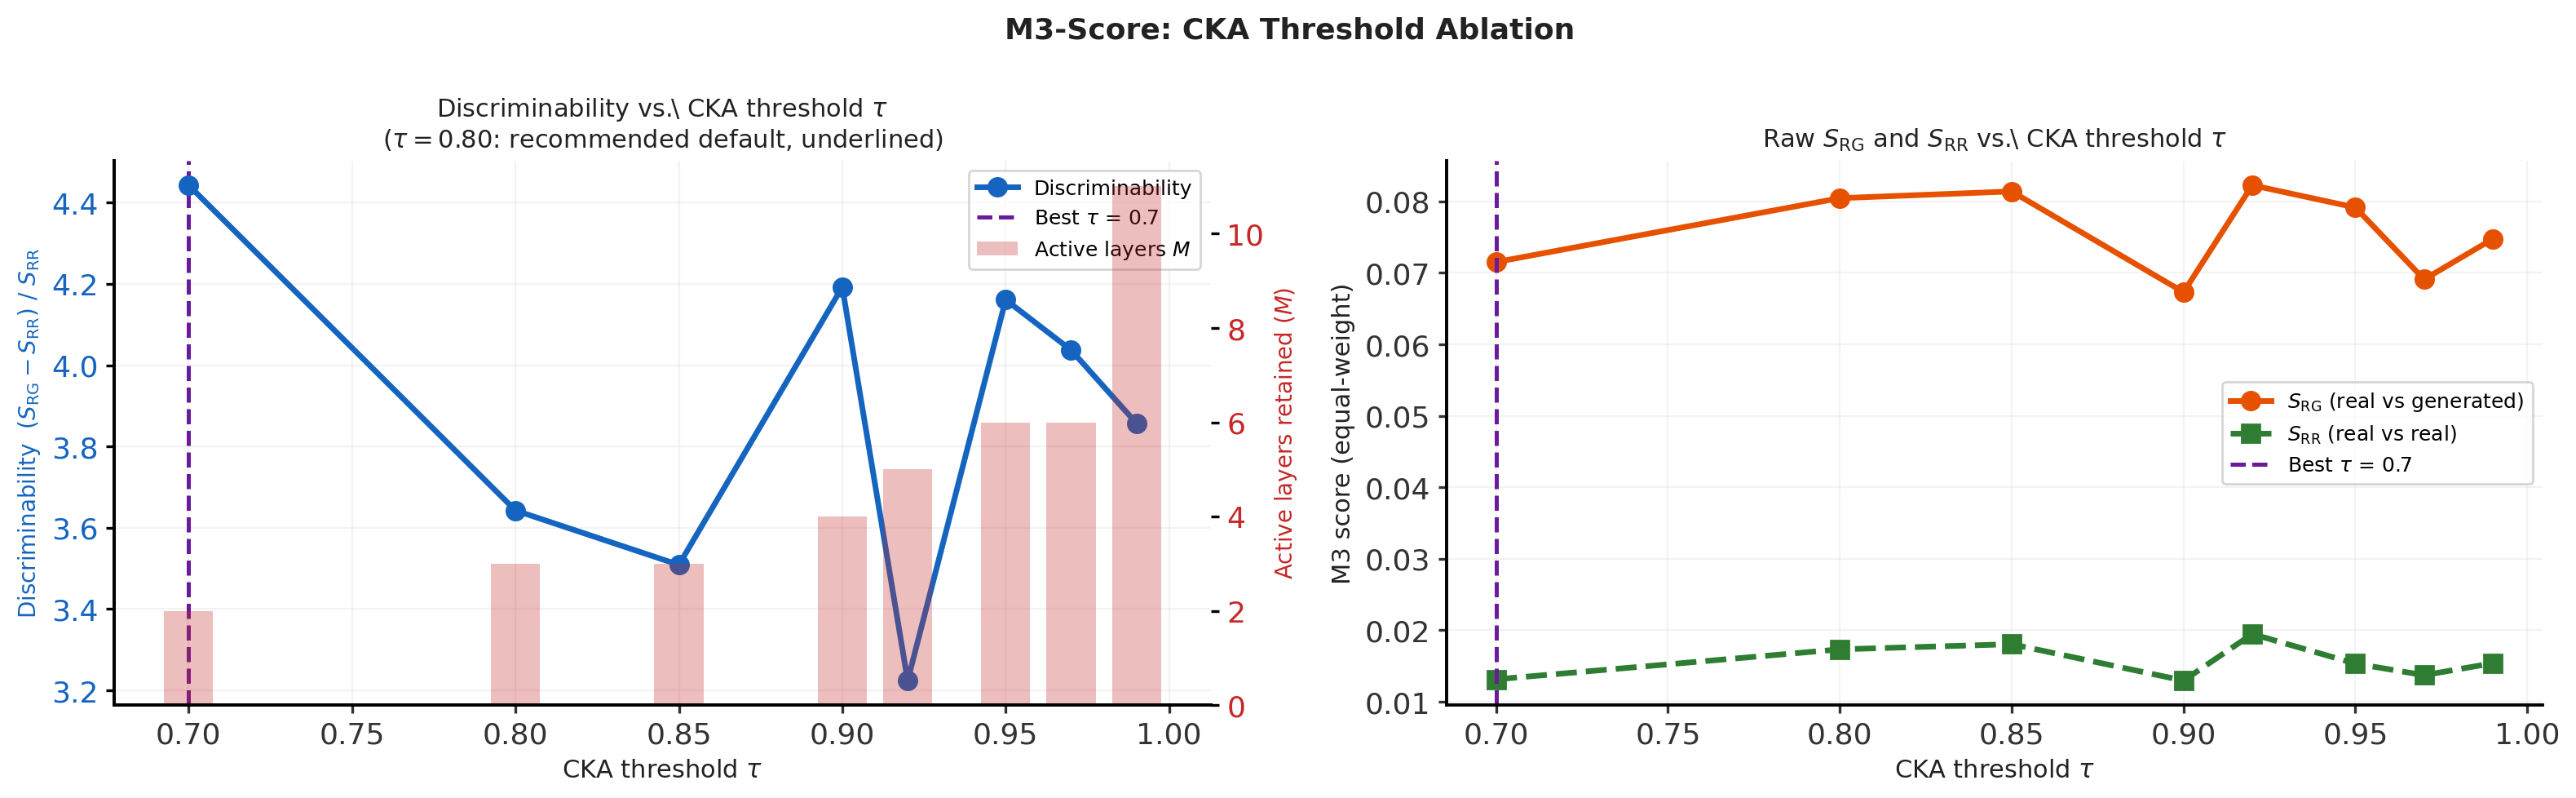
\includegraphics[width=0.9\textwidth]{Images/weight_abalation/weight_ablation_discriminability.png}

\caption{CKA threshold ablation ($N = 500$, CLS-token CKA). \emph{Left}: discriminability,
defined as $(S_{\mathrm{RG}} - S_{\mathrm{RR}})/S_{\mathrm{RR}}$ (blue, left axis),
and the number of active layers $M$ (red bars, right axis) versus threshold $\tau$.
The curve is non-monotonic: peak discriminability at $\tau = 0.70$
($M = 1$, discriminability $= 9.539$) uses only L12, while
$\tau = 0.80$ ($M = 2$, discriminability $= 9.423$)
adds L1. This confirms that
real-versus-generated separation is carried by the final layer.}

\label{fig:ablation}
\end{figure*}

% ------------------------------------------------------------
\subsection{Statistical Significance: Permutation Test}
\label{sec:results_permutation}
% ------------------------------------------------------------

We construct a null distribution by pooling the real and generated L12
fidelity features and permuting the labels $500$ times, recomputing the
unbiased MMD$^2$ on each shuffle (Section~\ref{sec:method_axes}). This is
the native fidelity-axis permutation test, not an auxiliary construction.

The observed fidelity MMD$^2$ is $0.153$. No permuted statistic out of $500$
reached it, giving an empirical $p < 0.002$ (the resolution floor at $500$
permutations), and the bootstrap $95\%$ confidence interval $[0.146,\ 0.162]$
excludes the null mean ($\approx 0$) by roughly two orders of magnitude.
For reference, the observed value lies $446$ permutation-null standard
deviations above the null mean ($\sigma_0 = 3.4\times10^{-4}$). We stress
that this ratio is a null-standardized separation magnitude, \emph{not} a
Gaussian $z$-score: it scales approximately linearly with $N$ because the
unbiased MMD$^2$ null variance shrinks as $O(1/N)$ while the observed
statistic converges to a positive constant, and the permutation null is
strongly non-Gaussian. Inference therefore rests on the permutation
$p$-value and the bootstrap interval, both of which establish separability
between the real and generated distributions well beyond conventional
thresholds and, unlike FID/KID/CMMD, are produced natively by the metric.


% =============================================================================
\section{Discussion}
\label{sec:discussion}
% =============================================================================

\paragraph{Why RadioDINO and not InceptionV3 or CLIP?}
Backbone alignment with the target domain is not a stylistic choice; it is a
prerequisite for sensitivity. InceptionV3 is trained on $1000$
natural-image classes and CLIP on web image-caption pairs. Neither has been
exposed to the systematic co-variation of tissue intensity, pathological
contrast, and acquisition artifact that defines a radiology distribution.
The clearest evidence is the CMMD rank inversion (Table~\ref{tab:cmmd_fail}):
CLIP features place the cross-modality CT shift \emph{closer} to real brain MRI
than a weak in-domain MRI generator ($\Delta_{\mathrm{CT}-\mathrm{MRI}}=-0.039$,
95\% CI $[-0.059,-0.021]$, excluding zero), whereas the radiology-trained
RadioDINO-s16 fidelity axis orders them correctly. The same backbone choice
yields the OOD-AUC margin ($0.976$ vs.\ $0.809$ for InceptionV3 and $0.659$ for
CLIP).

We stress that this is not a defect of the MMD estimator but a
\emph{misalignment of the CLIP embedding space with radiology modality
structure}. CLIP is trained to align images with free-text captions, so its
geometry is organised around high-level, modality-agnostic semantics
(``a medical scan of a brain/chest'') rather than the Hounsfield-unit,
tissue-texture, and acquisition statistics that govern pixel-level radiology
fidelity. Under that objective, a lung CT and a brain MRI can be nearer in
caption-semantic space than a brain MRI is to a \emph{degraded} brain MRI; the
CLIP embedding is doing exactly what it was trained to do. We therefore do not
claim CLIP fails at natural-image evaluation, nor that CMMD is incorrectly
implemented; we show that CLIP's text-alignment ontology is structurally unfit
for \emph{ordering} radiology fidelity, which is precisely the gap a
radiology-pretrained encoder closes.

\paragraph{On the a-priori layers and the discarded adaptive design}
An earlier version of this work selected layers adaptively by CKA pruning
and a discriminability criterion. We deliberately abandoned that design:
selecting a layer because it maximises measured separability is selection on
the test outcome, which inflates apparent performance. The canonical metric
now fixes L12/L9/L4 by representational position alone. The CKA ablation
(Section~\ref{sec:results_ablation}) is retained only to show that this
a-priori choice coincides with what an adaptive procedure would have picked
for the fidelity axis (L12 is retained at every threshold), so we lose
nothing by fixing it in advance and we gain immunity to outcome-driven
selection.

\paragraph{Where M3 does not win}
We emphasise three honest limitations. First, \emph{sample efficiency}: FID
is more stable than M3 for $N < 100$ (Table~\ref{tab:cv}); the unbiased
MMD$^2$ estimator pays for its lack of a Gaussian assumption with higher
small-sample variance, so M3 should be reported at $N \geq 100$. Second, the
\emph{coverage axis} is not yet a validated claim: under mode-drop it
behaves non-monotonically because $k$-NN radii inflate as the generated set
shrinks (Section~\ref{sec:results_axes}). Third, the \emph{lesion-specificity}
of M3 is real but narrow: with real expert masks it vanishes under gross
erasure and appears only under subtle degradation ($1.4$--$1.8\times$ vs.\ an
Inception baseline's $\sim$$1.05\times$; Section~\ref{sec:results_masking}). It
is therefore artifact \emph{specificity} to subtle, semantically meaningful
change, not the raw-sensitivity advantage claimed in early drafts. A study with
a lesion-conditioned generator is required to extend this from a
metric-sensitivity test to a generator-quality claim.

\paragraph{Limitations and scope}
M3-Score is validated primarily on brain MRI (BraTS), with cross-modality
checks on CT and retinal fundus. It is scoped to the radiology (CT/MRI)
domain: RadioDINO was trained on radiology, and our cross-modality ordering
shows M3 values are not comparable across the radiology boundary
(Section~\ref{sec:results_ood}). Extending validation to chest X-ray and CT
generators with ground-truth pathology masks is the principal direction for
future work.
The metric also requires inference through a 12-layer ViT-S/16, which
adds latency compared to FID: on a single consumer GPU the fidelity
$\mathrm{MMD}^2$ computation itself takes $\approx 8$\,s for $500$ images,
and $\approx 1$--$2$ minutes including the forward pass through the ViT for
feature extraction.
Finally, while $N = 500$ is standard for metric evaluation, larger-scale
($N \geq 1000$) and multi-site validation of the fidelity axis remains future
work.
Because the canonical metric fixes its layers a priori, it introduces no
layer-selection or weighting hyperparameter; the only sample-size guidance
is to use $N \geq 100$, since the unbiased MMD$^2$ estimator carries higher
variance at small $N$ (Table~\ref{tab:cv}) and can return small negative
values for $N < 50$.

\paragraph{Connection to existing metrics}
The three M3 axes are complementary to manifold-based metrics such as
Alpha-Precision and Beta-Recall. The fidelity axis measures
\emph{feature-level} shift with a domain-calibrated kernel and a native
significance test; the memorization axis targets near-duplicate leakage; the
coverage axis (with the caveats above) targets diversity. We recommend
reporting M3 alongside FID rather than in place of it: FID remains the more
sample-stable scalar at small $N$, while M3 adds radiology-domain
discrimination, the CMMD-style failure it avoids, and per-axis diagnostics.

% =============================================================================
\section{Conclusion}
\label{sec:conclusion}
% =============================================================================

We introduced the M3-Score, a radiology-domain evaluation framework for
generative image models built on the frozen RadioDINO-s16 ViT. Rather than a
single tuned scalar, M3 reports three axes read from layers fixed a priori by
representational depth: a fidelity axis (unbiased multi-bandwidth RBF
MMD$^2$ at L12) with a native permutation $p$-value, bootstrap CI, and
null-standardized separation $Z$; a memorization axis (L9) validated to recover injected
near-duplicate rates exactly; and a coverage axis (L4) that we report, with
explicit caveats, as a diagnostic still under development.
On BraTS brain MRI the fidelity axis separates real from generated images at
permutation $p < 0.002$ (bootstrap $95\%$ CI $[0.146,0.162]$ excluding zero)
and detects out-of-distribution radiology at
ROC-AUC $= 0.976$, versus $0.809$ for InceptionV3 and $0.659$ for CLIP. Our
central result is the structural failure of CMMD, which \emph{rank-inverts} a
cross-modality CT shift and a weak in-domain generator, placing CT closer to
real MRI (paired $\Delta = -0.039$, 95\% CI $[-0.059,-0.021]$, excluding
zero), where M3 (and FID) order them correctly.

We also report, rather than reinterpret, results that do not favour M3: FID
is more sample-stable at $N < 100$; the coverage axis is unstable under
$k$-NN radius inflation; and, with real expert lesion masks, M3 shows no
lesion-specific advantage under gross erasure and only a modest one
($1.4$--$1.8\times$) under subtle degradation: artifact specificity, not raw
sensitivity. The open-source implementation and a-priori layer configuration
are released for reproducibility. Future work will extend validation to chest
X-ray and CT generators, evaluate a lesion-conditioned generator against these
real masks, and place the coverage axis on a firmer footing at larger sample
sizes.

% =============================================================================
\appendices
\section{Legacy Adaptive Aggregation and CKA Layer Selection}
\label{app:legacy}
This appendix documents the \emph{superseded} adaptive design, retained only for the post-hoc validation reported in Section~\ref{sec:results_ablation}. It is \emph{not} part of the canonical M3-Score (Algorithm~\ref{alg:m3canonical}, Section~\ref{sec:method_axes}): the canonical fidelity, memorization, and coverage axes read the fixed layers $\{12,9,4\}$ and require none of the machinery below, so no layer, threshold, or weight is selected on test outcomes.

\begin{algorithm}[t]
\caption{Legacy adaptive M3 aggregation (optional post-hoc path) \newline \small{(CKA: Centered Kernel Alignment; MMD: Maximum Mean Discrepancy; ExtractFeat: Feature Extraction; Agg: Aggregation)}}
\label{alg:m3score}
\begin{algorithmic}[1]
\Require Real set $\mathcal{X}_r$, generated set $\mathcal{X}_g$,
         encoder $\Phi$ with $L$ layers,
         CKA threshold $\tau$, sub-batch count $K$,
         reference size $N_r \leq N$
\Ensure  Score $S$, layer distances
         $\{\widehat{\text{MMD}}^2_\ell\}_{\ell \in \mathcal{L}}$,
         layer weights $\{w_\ell\}_{\ell \in \mathcal{L}}$
\State $\mathcal{X}_r^{(N_r)} \leftarrow \{x_1, \ldots, x_{N_r}\}$
\State $\mathcal{L} \leftarrow
       \textsc{CKAPrune}(\Phi,\, \mathcal{X}_r^{(N_r)},\, \tau)$
       \Comment{Algorithm~\ref{alg:cka_pruning}}
\State $\{E_r^{(\ell)}\}_{\ell \in \mathcal{L}} \leftarrow
       \textsc{ExtractFeat}(\Phi,\, \mathcal{X}_r,\, \mathcal{L})$
       \Comment{Algorithm \ref{alg:extraction}}
\State $\{E_g^{(\ell)}\}_{\ell \in \mathcal{L}} \leftarrow
       \textsc{ExtractFeat}(\Phi,\, \mathcal{X}_g,\, \mathcal{L})$
\For{each $\ell \in \mathcal{L}$}
  \State $\widehat{\text{MMD}}^2_\ell \leftarrow
         \textsc{MMD2U}(E_r^{(\ell)},\, E_g^{(\ell)})$
         \Comment{Algorithm~\ref{alg:mmd}}
  \For{$k = 1, \ldots, K$}
    \State $\mathcal{I}_r \leftarrow$ sample $\lfloor N/K \rfloor$
           indices from $\{1,\ldots,N\}$ without replacement
    \State $\mathcal{I}_g \leftarrow$ sample $\lfloor N/K \rfloor$
           indices from $\{1,\ldots,N\}$ without replacement
    \State $\delta_k^{(\ell)} \leftarrow
           \textsc{MMD2U}(E_r^{(\ell)}[\mathcal{I}_r],\,
           E_g^{(\ell)}[\mathcal{I}_g])$
  \EndFor
  \State $\bar{\delta}^{(\ell)} \leftarrow
         \frac{1}{K}\sum_{k=1}^{K} \delta_k^{(\ell)}$
  \State $\sigma^{(\ell)} \leftarrow
         \Bigl(\frac{1}{K}\sum_{k=1}^{K}
         (\delta_k^{(\ell)} - \bar{\delta}^{(\ell)})^2\Bigr)^{1/2}$
  \State $\mathrm{SNR}_\ell \leftarrow
         \min\!\Bigl(
         \bar{\delta}^{(\ell)} /
         (\sigma^{(\ell)} + \varepsilon),\; 10^4
         \Bigr)$
\EndFor
\State $w_\ell \leftarrow
       \textsc{Agg}(\{E_r^{(\ell)}\},\,\{E_g^{(\ell)}\},\,
       \{\widehat{\mathrm{MMD}}^2_\ell\},\,\{\bar{H}^{(\ell)}\})$
       \Comment{Algorithm~\ref{alg:aggregation}: entropy$\times$stability$\times$uniqueness}
\State $S \leftarrow
       \sum_{\ell \in \mathcal{L}} w_\ell \cdot \widehat{\text{MMD}}^2_\ell$
\State \Return $S,\;
       \{\widehat{\text{MMD}}^2_\ell\}_{\ell \in \mathcal{L}},\;
       \{w_\ell\}_{\ell \in \mathcal{L}}$
\end{algorithmic}
\end{algorithm}

% ------------------------------------------------------------
\subsection{Post-Hoc Validation: CKA-Based Layer Analysis}
\label{sec:method_cka}
% ------------------------------------------------------------

\paragraph{Motivation}
Adjacent transformer layers in DINOv2-style encoders frequently learn representations of high mutual similarity, particularly in the early and final blocks \cite{kornblith2019cka}.
Including such layers would introduce correlated and computationally redundant contributions to the final score.
The CKA \cite{kornblith2019cka} is used to identify a non-redundant subset $\mathcal{L}$ of the available layers $L$.

\paragraph{Linear CKA}
Given two embedding matrices $E^{(\ell_1)}, E^{(\ell_2)} \in \mathbb{R}^{N_r \times D}$ extracted from a reference set of $N_r$ real images, linear CKA is
\begin{equation}
  \label{eq:cka}
  \mathrm{CKA}(E^{(\ell_1)}, E^{(\ell_2)})
  = \frac{\lVert \tilde{E}^{(\ell_1)\top}
                 \tilde{E}^{(\ell_2)} \rVert_F^2}
         {\lVert \tilde{E}^{(\ell_1)\top}
                 \tilde{E}^{(\ell_1)} \rVert_F^2
          \cdot
          \lVert \tilde{E}^{(\ell_2)\top}
                 \tilde{E}^{(\ell_2)} \rVert_F^2}^{1/2},
\end{equation}
where $\tilde{E}^{(\ell)} = E^{(\ell)} - \mathbf{1}\bar{e}^{(\ell)\top}$ is the column-centred matrix, $\bar{e}^{(\ell)} = \frac{1}{N_r}\sum_i E^{(\ell)}_{i,:}$ is the column mean, and $\lVert \cdot \rVert_F$ denotes the Frobenius norm. $\mathrm{CKA}(E^{(\ell_1)}, E^{(\ell_2)}) \in [0, 1]$, with value 1 indicating identical representational geometry.

Evaluating Eq.~\eqref{eq:cka} directly requires forming
$(D \times D)$ covariance matrices, whose denominator scales as
$\lVert \cdot \rVert_F^4 \sim D^4$ and is numerically unstable. Following
the HSIC reformulation in~\cite{kornblith2019cka}, we instead compute CKA
via $(N_r \times N_r)$ gram matrices, which are independent of feature
dimension:

\begin{align}
  K^{(\ell)} &= \tilde{E}^{(\ell)} \tilde{E}^{(\ell)\top}
               \in \mathbb{R}^{N_r \times N_r},
  \label{eq:gram} \\
  \mathrm{CKA}(\ell_1, \ell_2)
  &= \frac{\langle K^{(\ell_1)},\, K^{(\ell_2)} \rangle_F}
          {\lVert K^{(\ell_1)} \rVert_F \cdot
           \lVert K^{(\ell_2)} \rVert_F},
  \label{eq:cka_gram}
\end{align}
where $\langle A, B \rangle_F = \sum_{ij} A_{ij} B_{ij}$ is the
Frobenius inner product, proportional to the Hilbert-Schmidt
Independence Criterion.

\paragraph{Greedy backward selection}
Given $\tau \in (0, 1)$ (default $\tau = 0.80$), a greedy pass
iterating from layer $L-1$ to layer $1$ adds a layer to $\mathcal{L}$ only if its CKA similarity to every layer already in $\mathcal{L}$ is below $\tau$. Layer $L$ is always retained as the anchor. The full procedure is stated as Algorithm~\ref{alg:cka_pruning}.

On BraTS brain MRI with $\tau = 0.80$, the procedure selects
$M = 3$ layers $\mathcal{L} = \{1, 3, 12\}$, spanning early, mid, and
deep transformer blocks.
The number $M$ of retained layers is data-adaptive and varies with both
the imaging modality and the CKA threshold $\tau$; it is reported
alongside $S$ for reproducibility.
In the BraTS evaluation, layers 1, 3, and 12 are retained because their
pairwise CKA similarities all fall below $\tau = 0.80$, indicating that
each captures a distinct aspect of the radiology-specific feature
hierarchy~\cite{dosovitskiy2020vit,oquab2023dinov2}: early layers encode local texture and edge responses,
mid-network layers encode tissue boundaries and coarse anatomy, and
the final layer encodes semantic pathology structure.
CKA layer selection is performed once per evaluation session on
$N_r = 20$ images using CLS token features and the resulting $\mathcal{L}$
is reused for the full evaluation pass.

\begin{algorithm}[t]
\caption{CKA-based greedy layer selection ($\textsc{CKAPrune}$)}
\label{alg:cka_pruning}
\begin{algorithmic}[1]
\Require Encoder $\Phi$, reference set $\mathcal{X}_r^{(N_r)}$,
         threshold $\tau$
\Ensure  Active layer set $\mathcal{L} \subseteq \{1,\ldots,L\}$
\For{$\ell = 1, \ldots, L$}
  \State $E^{(\ell)} \leftarrow
         \textsc{ExtractFeatures}(\Phi,\,
         \mathcal{X}_r^{(N_r)},\, \{\ell\})$
  \State $\tilde{E}^{(\ell)} \leftarrow
         E^{(\ell)} - \mathbf{1}\bar{e}^{(\ell)\top}$
         \Comment{column-centre, Eq.~\eqref{eq:cka}}
  \State $K^{(\ell)} \leftarrow
         \tilde{E}^{(\ell)}\tilde{E}^{(\ell)\top}$
         \Comment{$(N_r \times N_r)$ gram matrix, Eq.~\eqref{eq:gram}}
\EndFor
\State $\mathcal{L} \leftarrow \{L\}$
       \Comment{layer $L$ is retained unconditionally}
\For{$\ell = L-1, L-2, \ldots, 1$}
  \State $\mathit{redundant} \leftarrow \mathrm{false}$
  \For{each $\ell' \in \mathcal{L}$}
    \State $\rho \leftarrow
           \langle K^{(\ell)},\, K^{(\ell')} \rangle_F \;/\;
           (\lVert K^{(\ell)} \rVert_F \cdot
            \lVert K^{(\ell')} \rVert_F)$
           \Comment{Eq.~\eqref{eq:cka_gram}}
    \If{$\rho > \tau$}
      \State $\mathit{redundant} \leftarrow \mathrm{true}$
      \State \textbf{break}
    \EndIf
  \EndFor
  \If{$\neg\,\mathit{redundant}$}
    \State $\mathcal{L} \leftarrow \mathcal{L} \cup \{\ell\}$
  \EndIf
\EndFor
\State \Return $\mathcal{L}$
\end{algorithmic}
\end{algorithm}

% ------------------------------------------------------------



% ------------------------------------------------------------
\subsection{Legacy Adaptive Aggregation (Superseded)}
\label{sec:method_aggregation}
% ------------------------------------------------------------

\emph{The weighting scheme below was the aggregation rule of the original
single-scalar M3 and is retained for completeness and reproducibility of the
post-hoc CKA validation. It is not used by the canonical three-axis metric
of Section~\ref{sec:method_axes}, which reports fidelity, memorization, and
coverage separately rather than collapsing them into one weighted sum. When
the CKA analysis reduces to the single most discriminative layer (L12), all
weighting schemes below coincide and the aggregate equals the fidelity axis.}

Not all retained layers in $\mathcal{L}$ contribute equally useful
information to the final score.
Three orthogonal criteria determine the weight assigned to each layer:
\emph{semantic focus} (does the layer attend to diagnostically relevant
image regions?), \emph{statistical stability} (is its MMD$^2$ estimate
consistent across sub-samples?), and \emph{representational uniqueness}
(does it capture aspects not already captured by another retained layer?).
The final weight for layer $\ell$ is proportional to the product of all
three components:
\begin{equation}
  \label{eq:weights}
  \tilde{w}_\ell
  = \mathrm{Sem}_\ell \cdot \mathrm{Stab}_\ell \cdot \mathrm{Uniq}_\ell,
  \qquad
  w_\ell = \frac{\tilde{w}_\ell}
                {\sum_{\ell' \in \mathcal{L}} \tilde{w}_{\ell'}}.
\end{equation}
Each component is defined and motivated below.

\paragraph{Semantic focus $\mathrm{Sem}_\ell$}
The CLS-to-patch attention weights
$\{\tilde{\alpha}^{(\ell)}_{b,p}\}$ (Eq.~\eqref{eq:attn_norm}) encode
which image patches the encoder considers most relevant at layer $\ell$.
When the attention is concentrated on a small number of patches, the
layer responds selectively to localised anatomical structures, which is
diagnostically informative for medical images.
When the attention is nearly uniform, the layer integrates all patches
equally and its features are less discriminative.
This selectivity is quantified by the Shannon entropy of the attention
distribution for image $b$,
\begin{equation}
  \label{eq:entropy}
  H^{(\ell)}_b =
  - \sum_{p=1}^{N_\mathrm{seq}-1}
    \tilde{\alpha}^{(\ell)}_{b,p}
    \log \tilde{\alpha}^{(\ell)}_{b,p},
\end{equation}
and the layer-level entropy is the mean over the real image set,
$\bar{H}^{(\ell)} = \frac{1}{N}\sum_{b=1}^{N} H^{(\ell)}_b$.
The semantic focus weight is defined as
\begin{equation}
  \label{eq:semanticity}
  \mathrm{Sem}_\ell = \exp\!\left(
    -\frac{\bar{H}^{(\ell)}}{T}
  \right),
\end{equation}
where $T > 0$ is a temperature parameter (default $T = 1$).
$\mathrm{Sem}_\ell \in (0, 1]$, approaching $1$ for a perfectly focused
layer and approaching $\exp(-\log(N_\mathrm{seq}-1)/T)$ for a perfectly
uniform layer.
The exponential form ensures that layers with very low entropy receive
substantially higher weight than layers with only moderately low entropy.

\paragraph{Statistical stability $\mathrm{Stab}_\ell$}
For each retained layer $\ell$, $K$ sub-batch MMD$^2$ estimates are
obtained by drawing independent random subsets of size
$n_k = \lfloor N/K \rfloor$ from both the real and generated embedding
matrices and evaluating Eq.~\eqref{eq:mmd} on each pair.
Denoting the $k$-th sub-batch estimate as $\delta_k^{(\ell)}$, the
mean and standard deviation of the sub-batch estimates are
\begin{align}
  \bar{\delta}^{(\ell)} &=
    \frac{1}{K}\sum_{k=1}^{K} \delta_k^{(\ell)}, \\
  \sigma^{(\ell)} &=
    \Bigl(\frac{1}{K}\sum_{k=1}^{K}
    \bigl(\delta_k^{(\ell)} - \bar{\delta}^{(\ell)}\bigr)^2
    \Bigr)^{1/2}.
\end{align}
The stability weight is the signal-to-noise ratio of the sub-batch
estimates, capped to prevent any single layer from monopolising the
total weight when its sub-batch variance is near zero:
\begin{equation}
  \label{eq:stability}
  \mathrm{Stab}_\ell =
  \min\!\left(
    \frac{\bar{\delta}^{(\ell)}}{\sigma^{(\ell)} + \varepsilon},\;
    10^4
  \right),
  \quad \varepsilon = 10^{-6}.
\end{equation}
The numerator $\bar{\delta}^{(\ell)}$ ensures that layers with a large
and consistent MMD$^2$ (clear distributional gap) receive higher
stability than layers with a large but highly variable MMD$^2$.
The cap of $10^4$ is necessary because $\sigma^{(\ell)} \to 0$ when all
sub-batches agree exactly (e.g.\ under zero perturbation), in which case
an uncapped inverse-variance weight would collapse the entire weight
distribution onto one layer regardless of its semantic or uniqueness
properties.
The default is $K = 5$; the sensitivity of $S$ to $K$ is reported in
Section~\ref{sec:results_ablation}.

\paragraph{Representational uniqueness $\mathrm{Uniq}_\ell$}
Although CKA pruning removes layers whose representations are highly
similar to any already-retained layer, the retained set $\mathcal{L}$
may still contain layers with moderate pairwise similarity.
To downweight such layers relative to those that capture genuinely
distinct aspects of the feature hierarchy, the uniqueness of layer
$\ell$ is defined as one minus its mean CKA similarity to all other
retained layers:
\begin{equation}
  \label{eq:uniqueness}
  \mathrm{Uniq}_\ell =
  \max\!\left(
  1 - \frac{1}{M - 1}
  \sum_{\substack{\ell' \in \mathcal{L} \\ \ell' \neq \ell}}
  \mathrm{CKA}(E_r^{(\ell)},\, E_r^{(\ell')}),\;
  10^{-4}
  \right),
\end{equation}
where $M = |\mathcal{L}|$ and CKA is evaluated on the real embedding
matrices via Eq.~\eqref{eq:cka_gram}.
$\mathrm{Uniq}_\ell \in (0, 1]$, approaching $1$ for a layer whose
representations are orthogonal to all other retained layers.
The floor of $10^{-4}$ prevents complete suppression of any layer.

\paragraph{Final score}
The unnormalised weight $\tilde{w}_\ell$ (Eq.~\eqref{eq:weights})
captures all three properties simultaneously: a layer receives high
weight only if it focuses on semantically relevant patches
($\mathrm{Sem}_\ell$ large), its MMD$^2$ estimate is consistent across
sub-samples ($\mathrm{Stab}_\ell$ large), and it is not redundant with
respect to the other retained layers ($\mathrm{Uniq}_\ell$ large).
The M3-Score is the weighted sum of the per-layer unbiased MMD$^2$
estimates:
\begin{equation}
  \label{eq:m3score}
  S = \sum_{\ell \in \mathcal{L}}
      w_\ell \cdot \widehat{\mathrm{MMD}}^2_\ell.
\end{equation}
Lower values of $S$ indicate greater distributional similarity between
the real and generated image sets.
$S = 0$ if and only if, for every $\ell \in \mathcal{L}$, the real and
generated embedding distributions are identical under the kernel $k$.
Algorithm~\ref{alg:aggregation} states the complete aggregation procedure.

\begin{algorithm}[t]
\caption{Entropy-stability-uniqueness aggregation}
\label{alg:aggregation}
\begin{algorithmic}[1]
\Require Real embeddings $\{E_r^{(\ell)}\}_{\ell \in \mathcal{L}}$,
         generated embeddings $\{E_g^{(\ell)}\}_{\ell \in \mathcal{L}}$,
         per-layer MMD$^2$ estimates $\{\widehat{\mathrm{MMD}}^2_\ell\}$,
         per-layer mean attention entropy $\{\bar{H}^{(\ell)}\}$,
         sub-batch count $K = 5$, temperature $T = 1$,
         SNR cap $C = 10^4$, floor $f = 10^{-4}$
\Ensure  Score $S$, normalised weights $\{w_\ell\}_{\ell \in \mathcal{L}}$
\For{each $\ell \in \mathcal{L}$}
  \State $\mathrm{Sem}_\ell \leftarrow
         \exp(-\bar{H}^{(\ell)} / T)$
         \Comment{semantic focus, Eq.~\eqref{eq:semanticity}}
  \For{$k = 1, \ldots, K$}
    \State $\mathcal{I}_r, \mathcal{I}_g \leftarrow$
           draw $\lfloor N/K \rfloor$ indices from $\{1,\ldots,N\}$
    \State $\delta_k^{(\ell)} \leftarrow
           \textsc{UnbiasedMMD2}(E_r^{(\ell)}[\mathcal{I}_r],\,
           E_g^{(\ell)}[\mathcal{I}_g])$
  \EndFor
  \State $\bar{\delta}^{(\ell)} \leftarrow
         \frac{1}{K}\sum_k \delta_k^{(\ell)}$
  \State $\sigma^{(\ell)} \leftarrow \bigl(
         \frac{1}{K}\sum_k (\delta_k^{(\ell)} -
         \bar{\delta}^{(\ell)})^2 \bigr)^{1/2}$
  \State $\mathrm{Stab}_\ell \leftarrow
         \min\!\bigl(\bar{\delta}^{(\ell)} /
         (\sigma^{(\ell)} + \varepsilon),\; C\bigr)$
         \Comment{capped SNR, Eq.~\eqref{eq:stability}}
  \State $\mathrm{Uniq}_\ell \leftarrow
         \max\!\bigl(1 - \frac{1}{M-1}
         \sum_{\ell' \neq \ell}
         \mathrm{CKA}(E_r^{(\ell)}, E_r^{(\ell')}),\; f\bigr)$
         \Comment{Eq.~\eqref{eq:uniqueness}}
  \State $\tilde{w}_\ell \leftarrow
         \mathrm{Sem}_\ell \cdot
         \mathrm{Stab}_\ell \cdot
         \mathrm{Uniq}_\ell$
         \Comment{unnormalised weight, Eq.~\eqref{eq:weights}}
\EndFor
\State $w_\ell \leftarrow
       \tilde{w}_\ell / \sum_{\ell'} \tilde{w}_{\ell'}$
       for all $\ell \in \mathcal{L}$
       \Comment{normalise}
\State $S \leftarrow
       \sum_{\ell \in \mathcal{L}} w_\ell \cdot
       \widehat{\mathrm{MMD}}^2_\ell$
       \Comment{Eq.~\eqref{eq:m3score}}
\State \Return $S,\; \{w_\ell\}_{\ell \in \mathcal{L}}$
\end{algorithmic}
\end{algorithm}



\bibliographystyle{IEEEtran}
\bibliography{IEEEabrv,refs}

\vfill

\end{document}